\documentclass[twocolumn,a4paper,10pt]{article}

\usepackage[utf8]{inputenc}
\usepackage[english]{babel}
\usepackage[T1]{fontenc}
%%%%%% MISE EN PAGES %%%%%%
\usepackage[width=175mm, top=3cm]{geometry}

\setcounter{tocdepth}{3}     % Dans la table des matieres
\setcounter{secnumdepth}{4}  % Avec un numero.

% \renewcommand{\chaptermark}[1]{\markboth{\thechapter.\space#1}{}} 
\usepackage{layout}

%%%%%% SYMBOLES %%%%%
\usepackage{tipa}	% pour avoir l'accent concave
\usepackage{lmodern}	% pour les guillemets
\usepackage{nth}

%%%%%% EQUATION %%%%%%
\usepackage{amssymb}
\usepackage{amsmath}
\usepackage{fancybox}
\usepackage{xfrac}	% fraction de type "1/4"
\usepackage{cases}	% système équation
\usepackage[overload]{empheq}
\usepackage{bm}		% pour mettre en gras .
\usepackage{units} 	% x/y barre latérale pour les fractions

%%%%%% FIGURE %%%%%%
\usepackage{graphicx}	% insérer des graphiques
\usepackage{subfigure}	% utiliser subfigure
\usepackage{float}	% utiliser H dans les figures

%%%%%% TABLEAUX %%%%%%
\usepackage{array,multirow,makecell}
%\addto\captionsfrench{\def\tablename{\textsc{Tableau}}}% pour avoir TABLEAU et pas TABLE dans les légendes des tableaux
\usepackage[table,xcdraw]{xcolor} % pour avoir des lignes colorées dans les tableau
\usepackage{slashbox} % pour les \backslashbox
%\usepackage{subcaption}
\usepackage{hhline}	% pour les lignes horizontales 
\usepackage{tabularx} % permet itemize dans les cellules


\newcolumntype{L}[1]{>{\raggedright\let\newline\\\arraybackslash\hspace{0pt}}m{#1}}
\newcolumntype{C}[1]{>{\centering\let\newline\\\arraybackslash\hspace{0pt}}m{#1}}
\newcolumntype{R}[1]{>{\raggedleft\let\newline\\\arraybackslash\hspace{0pt}}m{#1}}

%%%%%%%%%%%%%%%%%%%%%
\usepackage{url}	% gérer les adresses www.
\linespread{1}	% interligne

\cleardoublepage

\newcommand{\ml}[1]{\textcolor{blue}{ Mathieu: #1}}

\title{Estimation of the road traffic sound levels in urban areas based on non-negative matrix factorization techniques}

\author{
    Jean-Rémy GLOAGUEN\\
    Arnaud Can\\
    LAE\\
    Ifsttar\\
    jean-remy.gloaguen@ifsttar.fr
  \and
    Mathieu Lagrange\\
	Jean-François Petiot \\
    LS2N, CNRS\\
    \'Ecole Centrale de  Nantes\\
}
\date{}
\begin{document}

\maketitle

\section*{Abstract}

The advent of low cost acoustic monitoring devices raises new interesting approaches for improving the monitoring of the acoustic quality of urban areas. State of the art approaches target road traffic noise maps and consider, as input, an estimate of the number and the speed of vehicles in major traffic lanes. Follows a prediction procedure that outputs an acoustic pressure level at any location in the modeled area.

Considering as input the acoustic pressure measured in many locations using a sensor grid approach would greatly complement and improve the quality of the predicted pressure values. Among the technical issues that raise this kind of innovative approaches, there is a need to identify which part of the overall acoustic pressure level is due to the road traffic.

In this paper, several techniques based on non-negative factorization framework are studied in this application scenario on a simulated sound scene corpus. The task being to the best of our knowledge never been considered in the literature, we propose an experimental protocol to validate the studied approaches that complies with standard reproducible research recommendations. The results shows the interest of our proposed approach for a such sound environment as it improves the estimation of the road traffic sound level with a lowest error compared to basic methods. 

\section{Introduction}

With the introduction of the European Directive 2002/EC/49, cities over 100 000 inhabitants have to produce road traffic noise maps. These maps depict the sound level distribution over the city and an estimation of the number of city dwellers exposed to high noise levels. These maps play both an important communication role and help drawing up action plans to reduce noise exposure. Road traffic noise maps are the result of a simulation process based on the estimation of the traffic density on the main roads and the use of sound propagation modelling. They express as output $L_ {DEN}$ and $L_N$ values, which are \textit{Day-Evening-Night} and \textit{Night} equivalent A-weighted sound levels respectively. Altough very useful, the produced noise maps introduce lot of uncertainty generated by the numerical tools \cite{van_leeuwen_noise_2015} or by the different calculation methodologies used \cite{leroy_uncertainty_2010}\cite{garg_critical_2014}, despite the long data collection and calculation times. In addition, the usual road traffic noise maps are static, aggregating the exposure into indicators $L_{DEN}$ and $L_N$, that ignore the sound levels evolution throughout the day. 
The use of acoustic measurements could facilitate their updating or even the generation of dynamic maps \cite{wei_dynamic_2016}. These measurements can be performed at fixed stations spread all over the cities \cite{Mioduszewski} \cite{mietlicki2012innovative}, which would make available of the long-term evolution of the traffic noise levels. It can also be performed with  mobile stations \cite{can_exploring_2012} \cite{manvell2004sadmam} covering a larger area with fewer sensors but also sparse time periods.

Currently, sensor networks in cities are spread for multiple applications (air quality assessment, measurement of meteorological parameters ...), including the assessment of urban noise levels. The DYNAMAP project \cite{dynamap_2016} studied the deployment and feasibility of such installations focusing on sensor installations on specific roads at the city scale in Milan and Rome \cite{bellucci_life_2017}. 
The SONYC project (Sounds Of New-York City) aims to deploy a sensor network in New-York City for the purpose of monitoring constantly the noise pollution in the city \cite{mydlarz2017implementation}. In order to better know the urban sound environment, sensors are coupled with a detection tool that identifies the sound sources present \cite{salamon2017deep}. In a similar way, but reduced to few neighborhoods with a denser network, the CENSE project\footnote{\url{http://cense.ifsttar.fr/}} \cite{picaut2017characterization} aims to combine \textit{in situ} observations, from a sensor network, and numerical data, from noise modeling, through data assimilation techniques.

Prior to data assimiliation, the issue of the correct estimation of the traffic sound level from acoustic measurements is still unsolved \cite{Mioduszewski}. Mainly because the urban sound environment is a complex environment gathering lots of different sounds (car passages, voices, whistling bird, car horn, airplanes\dots) that overlap. Consequently, the traffic sound level estimation based on measurements is not a trivial task.
Many recent works have focused on the detection or recognition tasks of environmental sounds \cite{heittola_sound_2011}, \cite{defreville_automatic_2006}, \cite{dufaux_automatic_2000}, \cite{chu_environmental_2009}. A two-step process is generally followed : describe the audio files with a set of features (Spectral Centroid, harmonicity, Mel-Frequency Cepstral Coefficient \dots) and classify them with the help of classifiers (Support Vector Machines, Gaussian Mixture Models, Hidden Markov Model, Artifical Neural Networks). A description of these features and classifiers can be found in \cite{cowling_comparison_2003} and their applications can be found in \cite{shen_environmental_2012}, \cite{beritelli_pattern_2008}, \cite{couvreur_automatic_2004}.

The main issue in the detection or recognition tasks is the overlap of environmental sounds. Although near major roads, traffic is predominant, there are many places where it overlaps with other sound sources which contribute significantly to the overall sound levels. To circumvent this issue, Socoro et al. propose to suppress time frames where there is significant overlap by considering an Anomalous Noise Events Detector \cite{socoro_anomalous_2017}. It consists in detecting the unwanted sound sources from labeled recordings, \textit{i.e.} that are not related to the traffic component. Those time frames are then discarded in order not to take them into account during the estimation of the traffic sound level. 
An alternative approach that we will follow in this paper is to consider the blind source separation paradigm to reliably estimate the traffic noise level, see Figure \ref{fig:diagram}. It consists in separating the contribution of the traffic from the other sources within a polyphonic scene. One major advantage of following such approach is that the estimate is continuously available, making the approach applicable in a wide range of urban areas, even where the traffic noise is relatively low compared to the remaining contributions.\\

In an urban environment context, source separation can be achieved with the help of acoustic microphone arrays and beamforming \cite{saruwatari2003blind}. However, this approach requires spreading multiple microphones arrays in cities that is very expensive (even with low cost microphones) and time-consuming for calibration and maintenance. This method is then not considered here to be deployed all over cities. In the opposite, monophonic sensor networks need less microphones but the main challenge is to succeed to estimate correctly the road traffic from only one signal in which all kind of sound sources can be present. A convenient method for this is the  Non-negative Matrix Factorization (NMF) technique \cite{lee_learning_1999}. When considering audio as input, it usually consists in approximating the magnitude spectrogram of an audio file by the product of two low rank matrices, one representing the components of interest and the other the contribution at a given time of those components to approximate the input magnitude spectrogram \cite{smaragdis_non-negative_2003} \cite{wilson_speech_2008} \cite{mesaros_sound_2015}. In the audio processing domain, NMF has already been employed for the source separation task of monaural signals of speech and music \cite{wang_musical_2005} \cite{wilson_speech_2008}. By design, this method deals reasonably well with the overlapping sound sources as soon as the overlap can be resolved on the time/frequency plane. 
Closer to our application scenario, NMF has been considered by Innami and Kasai \cite{satoshi_innami_nmf-based_2012}. After having performed NMF on simulated audio files, they perform a source separation in two steps by 1) separating the sound background from the events and 2) by isolating the events using spectral features using a $k$-means procedure.
We study in this paper different flavors of Non-Negative Matrix Factorization where the traffic component is considered in its entirely whether it is a sound background or an event. We demonstrate that supervised NMF and semi supervised NMF approaches have some interests but fail to give satisfactory results for the application at hand. We thus introduce another NMF scheme called thresholded initialized NMF that makes good use of prior knowledge about the source of interest, in our case the traffic noise, but also generalizes well to several kinds of urban areas and to traffic to interference ratio (TIR).

To perform the numerical experiments, we consider a corpus of simulated sound scenes created from a built-up sound database composed of a high number of diverse sound samples. The use of simulated sound scenes is mandatory for rigorous experimental validation as it offers a high level of control on the design of the scenes and the knowledge of the exact contribution of the traffic component ($L_{p,traffic}$), which would be difficult to extract from a recording of an urban scene.

\begin{figure*}[t]
\centering
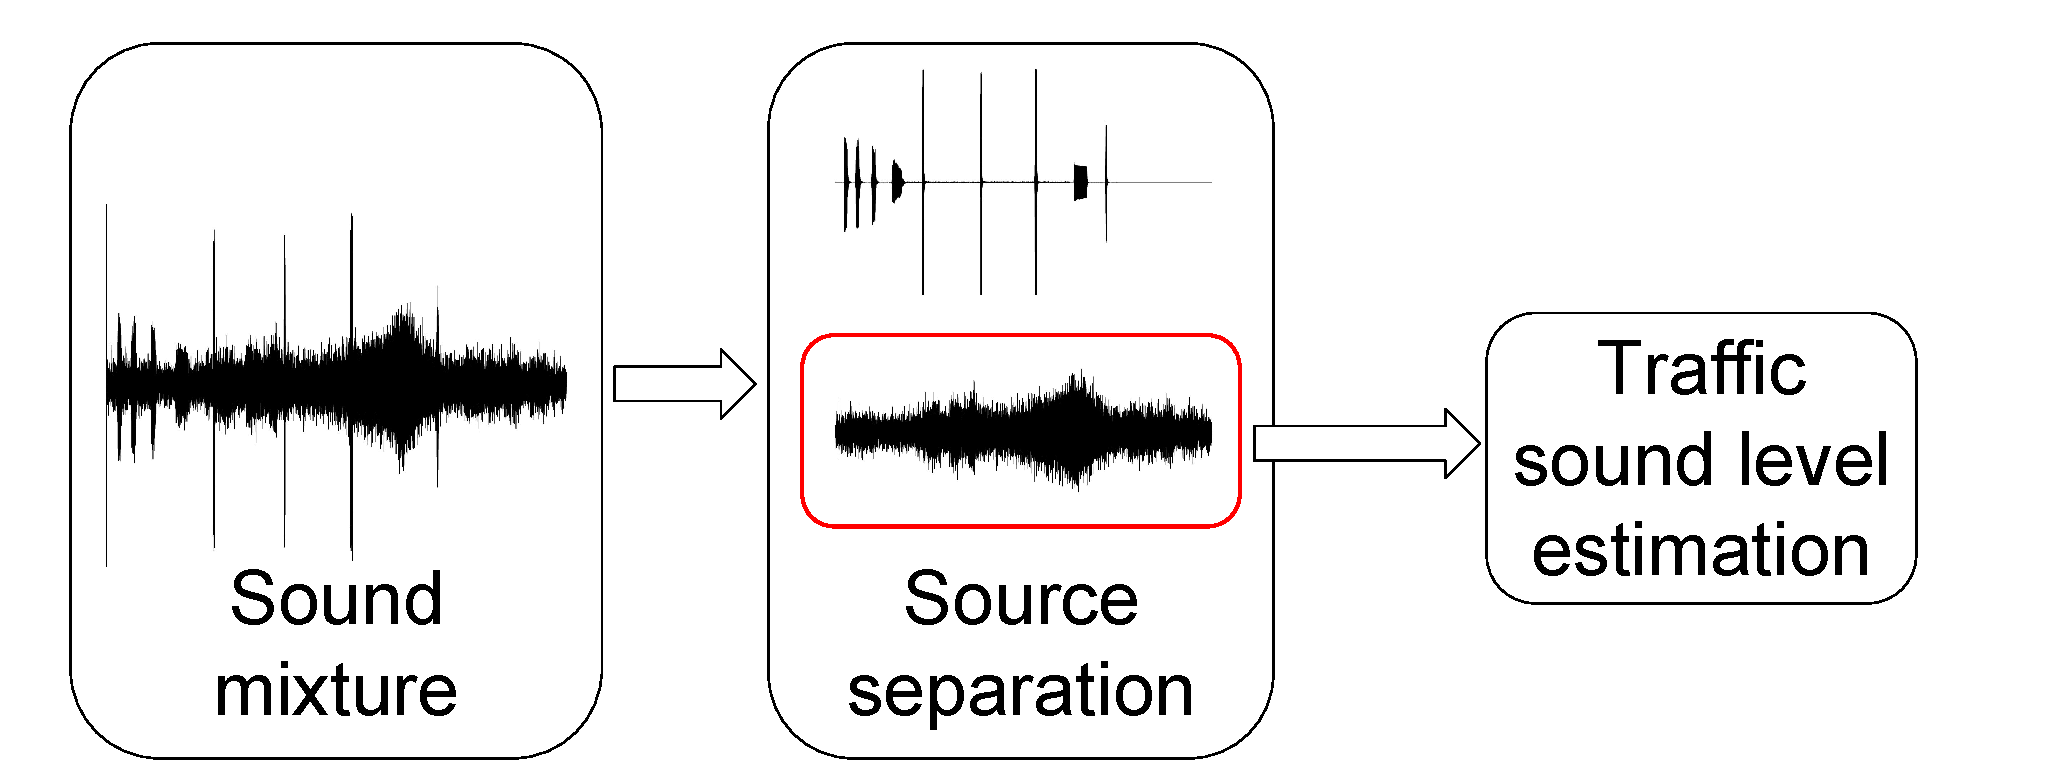
\includegraphics[width=0.7\textwidth]{figures/bloc_diagram_source_separation.pdf}
\caption{Block diagram of the general source separation model}
\label{fig:diagram}
\end{figure*}

The remaining of the paper is organized as follows. Section \ref{part:nmf} details the technical aspects of NMF and describes the 3 approaches considered in this paper to achieve the task at hand. Section \ref{part:protocol} describes the corpus of environmental sound scenes and the experimental protocol setup. Section \ref{part:results} presents and discusses the outcomes of the numerical results.

\section{Non-negative Matrix Factorization}\label{part:nmf}
\subsection{Description of NMF}

Non-negative Matrix Factorization is a linear approximation method introduced by Lee and Seung, \cite{lee_learning_1999}, which can be used to approximate the spectrogram $\mathbf{\tilde{V}}$ (obtained using a Short-Term Fourier Transform) of an audio file, $\mathbf{V}$, $\in \mathbb{R}^+_{F \times N}$ as :

\begin{equation}\label{eq:nmf}
\mathbf{V} \approx \mathbf{\tilde{V}} = \mathbf{WH}
\end{equation}

where $\mathbf{W} \in \mathbb{R}^+_{F \times K}$ is the \textit{dictionary} (or basis) matrix composed of audio spectra and $\mathbf{H} \in \mathbb{R}^+_{K \times N}$ is the \textit{activation} matrix which summarizes the temporal evolution of each element of $\mathbf{W}$. An illustrative example can be found in Figure  \ref{fig:example_NMF}.

\begin{figure}[t]
\centering
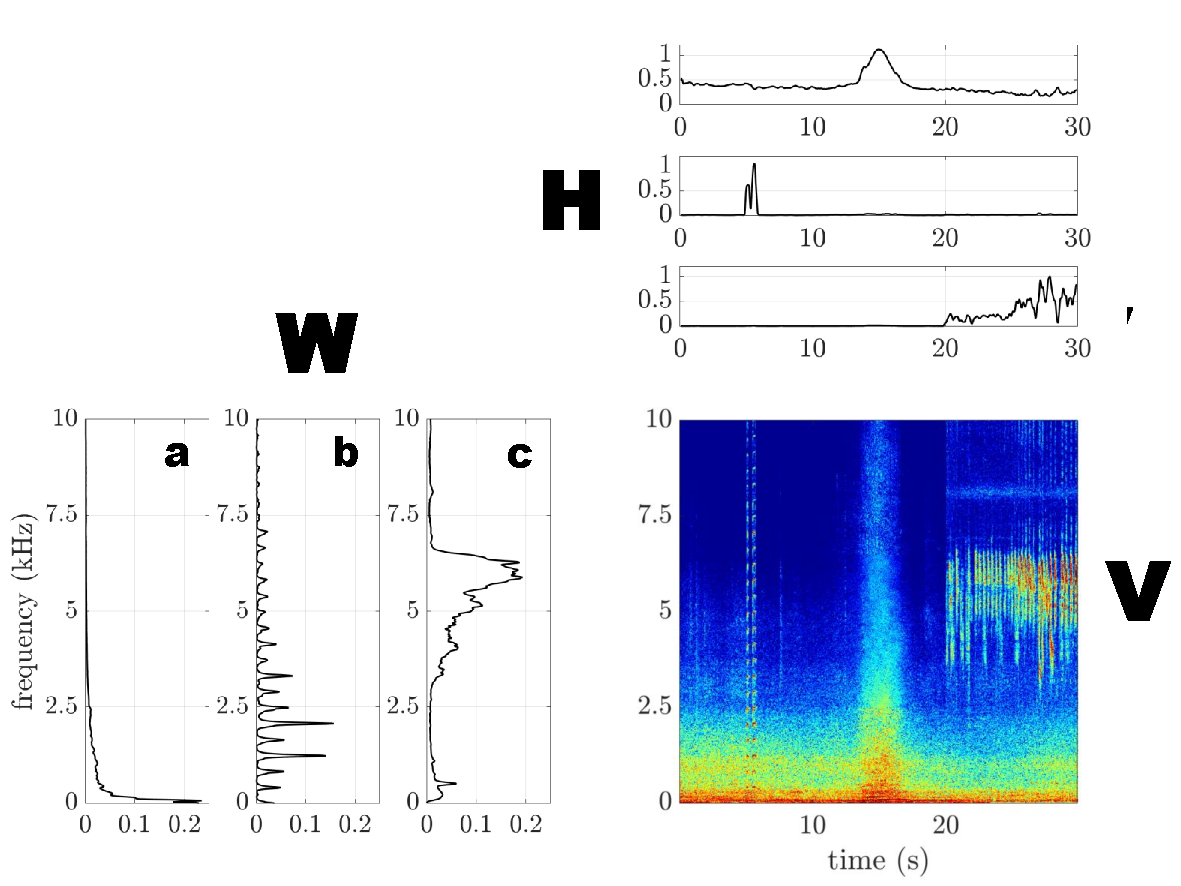
\includegraphics[width=0.9\linewidth]{figures/schema_introduction_nmf_2.pdf}
\caption{Example of a simple NMF for urban sound mixture composed of 3 sound events (car passages, car horn and bird's whistles), $\mathbf{W}$ is composed of 3 elements too ($K$ = 3) which correspond in 3 audio spectra (car passages (a), car horn (b) and bird's whistles (c))}
\label{fig:example_NMF}
\end{figure}

The choice of the dimensions is often made so that $F\times K + K \times N < F \times N$. NMF is then considered as a low rank approximation method. However, this constraint is not mandatory. To estimate the quality of the approximation, an objective function is used

\begin{equation}\label{eq:min-D-WH}
\underset{\mathbf{H} \geq 0, \mathbf{W} \geq 0}{\min} D\left(\mathbf{V} \vert \vert \mathbf{\tilde{V}}\right).
\end{equation}

The operator $D(x\vert y)$ is a divergence calculation such as:
\begin{equation}
D\left(\textbf{V} \vert\vert \mathbf{\tilde{V}} \right) = \sum_{f = 1}^{F} \sum_{n = 1}^{N} d_{\beta}
\left(\textbf{V}_{fn} \vert \left[ \textbf{WH} \right]_{fn} \right)
\end{equation}

and usually belongs to the $\beta-$divergence class \cite{fevotte_nonnegative_2009} in which the well known Euclidean distance (eq. \ref{eq:def_distEUC}) and the Kullback-Leibler divergence (eq. \ref{eq:def_divKL}) belong

\begin{subequations}\label{eq:divBetaGenerale}
\begin{numcases}{d_{\beta}(x\vert y) =}
    \frac{1}{2}(x-y)^2, & $\beta = 2$, \label{eq:def_distEUC}\\
    x\log \dfrac{x}{y} - x + y, & $\beta = 1$.\label{eq:def_divKL}
\end{numcases}
\end{subequations}

To better take into account prior knowledge about the sources of interest, constraints (like the smoothness or the sparsness criteria \cite{virtanen_monaural_2007}) can be added to the objective function.

Algorithms have been proposed to solve the minimization problem (\ref{eq:min-D-WH}) iteratively such as the multiplicative update \cite{lee_algorithms_2000}, the alternating least square method \cite{cichocki_regularized_2007} or the projected gradient \cite{lin_projected_2007}. Here, the multiplicative update is chosen as it ensures convergence as proven in \cite{fevotte_algorithms_2011}.

\subsection{Supervised NMF}
First, supervised NMF (Sup-NMF) is used: the \textit{dictionary} includes audio spectra of urban sound sources. A lot of the different sound sources present in the urban environment are known. Their spectra can be obtained and be a basis of $\mathbf{W}$. The \textit{activation} matrix is then the unknown variable to estimate. In the first iteration, $\mathbf{H}$ is initialized randomly, then it is updated by the generic algorithm \cite{fevotte_algorithms_2011}

\begin{equation}\label{eq:updateH_Sup}
\textbf{H}^{(i+1)} \leftarrow \textbf{H}^{(i)}.\left(\frac{\textbf{W}^T \left[\left(\textbf{WH}^{(i)} \right)^{(\beta-2)}.\textbf{V} \right]}{\textbf{W}^T \left[\textbf{WH}^{(i)} \right]^{(\beta-1)}}\right)^{\gamma(\beta)}
\end{equation}

with $\gamma(\beta) = \frac{1}{2-\beta},$ for $\beta < 1$, $ \gamma(\beta) = 1$, for $\beta \in \left[1,2\right]$ and $\gamma(\beta) = \frac{1}{\beta-1}$ for $\beta > 2$. The product $A.B$ and $A/B$ are respectively the Hadamard product and ratio. As in the supervised approach the indexes of traffic components in $\mathbf{W}$  are known, the separation of the corresponding sound source is made by extracting the related basis and activators,

\begin{equation}\label{eq:separationExtraction}
\mathbf{\tilde{V}}_{traffic} = \left[ \mathbf{WH} \right]_{traffic}.
\end{equation}

\subsection{Semi-supervised NMF}

The supervised approach is useful when prior knowldge can be assumed for all the sources in the mixture, which is not a reasonable assumption in our application scenario. To some extend, prior knowledge can be considered for the traffic but not for the numerous kind of interferences that can occur in a realistic scenario. To better take into account the diverse nature of urban scenes, semi-supervised NMF (Sem-NMF)\cite{lee_semi-supervised_2010} is a good candidate as it offers more flexibility. This method assumes a \textit{dictionary} with a fixed part $\mathbf{W_s} \in \mathbb{R}^+_{F\times K}$, composed in our case of road traffic spectra, and with a mobile part, $\mathbf{W_r} \in \mathbb{R}^+_{F\times J}$ with $J <<K$, that is updated during optimization. In the literature, $J$ is set to a small number with respect to $K$ so as to force the optimization to still consider the fixed part of the dictionary %\cite{fevotte ?}
. The aim is to include in $\mathbf{W_r}$ the elements that are not related with the traffic. The problem (\ref{eq:nmf}) becomes

\begin{equation}
\mathbf{V} \approx \mathbf{\tilde{V}} = \mathbf{W_s H_s}+ \mathbf{W_r H_r}
\end{equation}

 with $\mathbf{W} = \left[\mathbf{W_s} \mathbf{W_r} \right]$ and $\mathbf{H} = \genfrac[]{0pt}{0}{\mathbf{H_s}}{\mathbf{H_r}}$. In a similar way as to solve the equation (\ref{eq:min-D-WH}), $\mathbf{W_r}$, $\mathbf{H_r}$ and $\mathbf{H_s}$ are successively updated with the relations (\ref{eq:WH-SSupdate}):

{\scriptsize
\begin{subequations}\label{eq:WH-SSupdate}
\begin{align}
\mathbf{W_r}^{(i+1)} &\leftarrow \mathbf{W_r}^{(i)}.\left(\frac{\left[\left(\mathbf{W_r H_r}^{(i)} \right)^{(\beta-2)}.\mathbf{V} \right]\mathbf{H_r}^T}{\left(\mathbf{W_r H_r}^{(i)} \right)^{(\beta-1)}\mathbf{H_r}^T}\right)^{\gamma(\beta)}, \label{eq:W_r_SS}\\
\mathbf{H_r}^{(i+1)} &\leftarrow \mathbf{H_r}^{(i)}.\left(\frac{\mathbf{W_r}^T \left[\left(\mathbf{W_r H_r}^{(i)} \right)^{(\beta-2)}.\mathbf{V} \right]}{\mathbf{W_r}^T \left(\mathbf{W_r H_r}^{(i)} \right)^{(\beta-1)}}\right)^{\gamma(\beta)}, \label{eq:H_r_SS}\\
\mathbf{H_s}^{(i+1)} &\leftarrow \mathbf{H_s}^{(i)}.\left(\frac{\mathbf{W_s}^T \left[\left(\mathbf{W_s H_s}^{(i)} \right)^{(\beta-2)}.\mathbf{V} \right]}{\mathbf{W_s}^T \left(\mathbf{W_s H_s}^{(i)} \right)^{(\beta-1)}}\right)^{\gamma(\beta)}.\label{eq:H_s_SS}
\end{align}
\end{subequations}}

Applications of Sem-NMF for speech denoising from background noise or musical content can be found in \cite{joder2012real} and \cite{weninger2012supervised}.

\subsection{Thresholded initialized NMF}

As it will be demonstrated in the experimental results described in Section \ref{part:results}, those last approaches fail to provide consistent results in a wide range of urban areas and for different traffic preponderances due to generalization capabilities issues.

We therefore propose an alternative scheme based on the unsupervised NMF. Usually in unsupervised, $\mathbf{W}$, as  $\mathbf{H}$, are initialized randomly. Here, as the concerned sound source is known and audio samples of car passages are available, an initial dictionary, $\mathbf{W_0}$, is learnt by converting the audio files in the spectra domain; see part \ref{part:dictionary_learning}. Then NMF is performed where $\mathbf{W}$ (eq. \ref{eq:updateW_unsup}) and $\mathbf{H}$ (eq.  \ref{eq:updateH_Sup}) are updated alternatively. $\mathbf{W}$ is therefore updated by forcing its initiation with \textit{a priori} knowledge but allowing it to adapt to the actual content of the scene under study, 

\begin{equation}\label{eq:updateW_unsup}
\textbf{W}^{(i+1)} \leftarrow \mathbf{W}^{(i)}.\left(\frac{\left[\left(\mathbf{W}^{(i)}\mathbf{H} \right)^{(\beta-2)}.\mathbf{V} \right]\mathbf{H}^T}{\left[\mathbf{W}^{(i)}\mathbf{H} \right]^{(\beta-1)}\mathbf{H}^T}\right)^{\gamma(\beta)}.
\end{equation}

After $N$ iterations, a measure of similarity $D_{\theta}\left(\mathbf{W_0} \vert \vert \mathbf{W} \right)$ between $\mathbf{W_0}$ and the obtained dictionary $\mathbf{W}$ for each element $k$ is computed using a cosine similarity metric,

\begin{equation}
D_{\theta}\left(\mathbf{W_0}_k \vert \vert \mathbf{W}_k \right) = \frac{\mathbf{W_0}_k.\mathbf{W}_k}{\vert \vert \mathbf{W_0}_k  \vert \vert . \vert \vert \mathbf{W}_k \vert \vert}.
\end{equation}

$D_{\theta}\left(\mathbf{W_0}_k \vert \vert \mathbf{W}_k \right) = 1$ means that the elements are identical (the $k$-th element of $\mathbf{W}$ is then considered as traffic element) whereas $D_{\theta}\left(\mathbf{W_0}_k \vert \vert \mathbf{W}_k \right)$ = 0 means that the elements are completely different. This measure is bounded between 1 and 0 and is an invariant with respect to scale. The $k$ value of $D_{\theta}\left(\mathbf{W_0} \vert \vert \mathbf{W} \right)$ are next sorted in descending order. The elements in $\mathbf{W}$ that can belong to $\mathbf{W}_{traffic}$ are selected by a \textit{hard thresholding} method. It is defined as:

\begin{equation}
\mathbf{W}_k \in \mathbf{W}_{k,traffic} \quad \text{iff} \quad D\left(\mathbf{W_0}_k \vert \vert \mathbf{W}_{k} \right) > t.
\end{equation}

An illustrative example is shown in Figure \ref{fig:W_TI_NMF}.\\

\begin{figure}[hbtp]
\centering
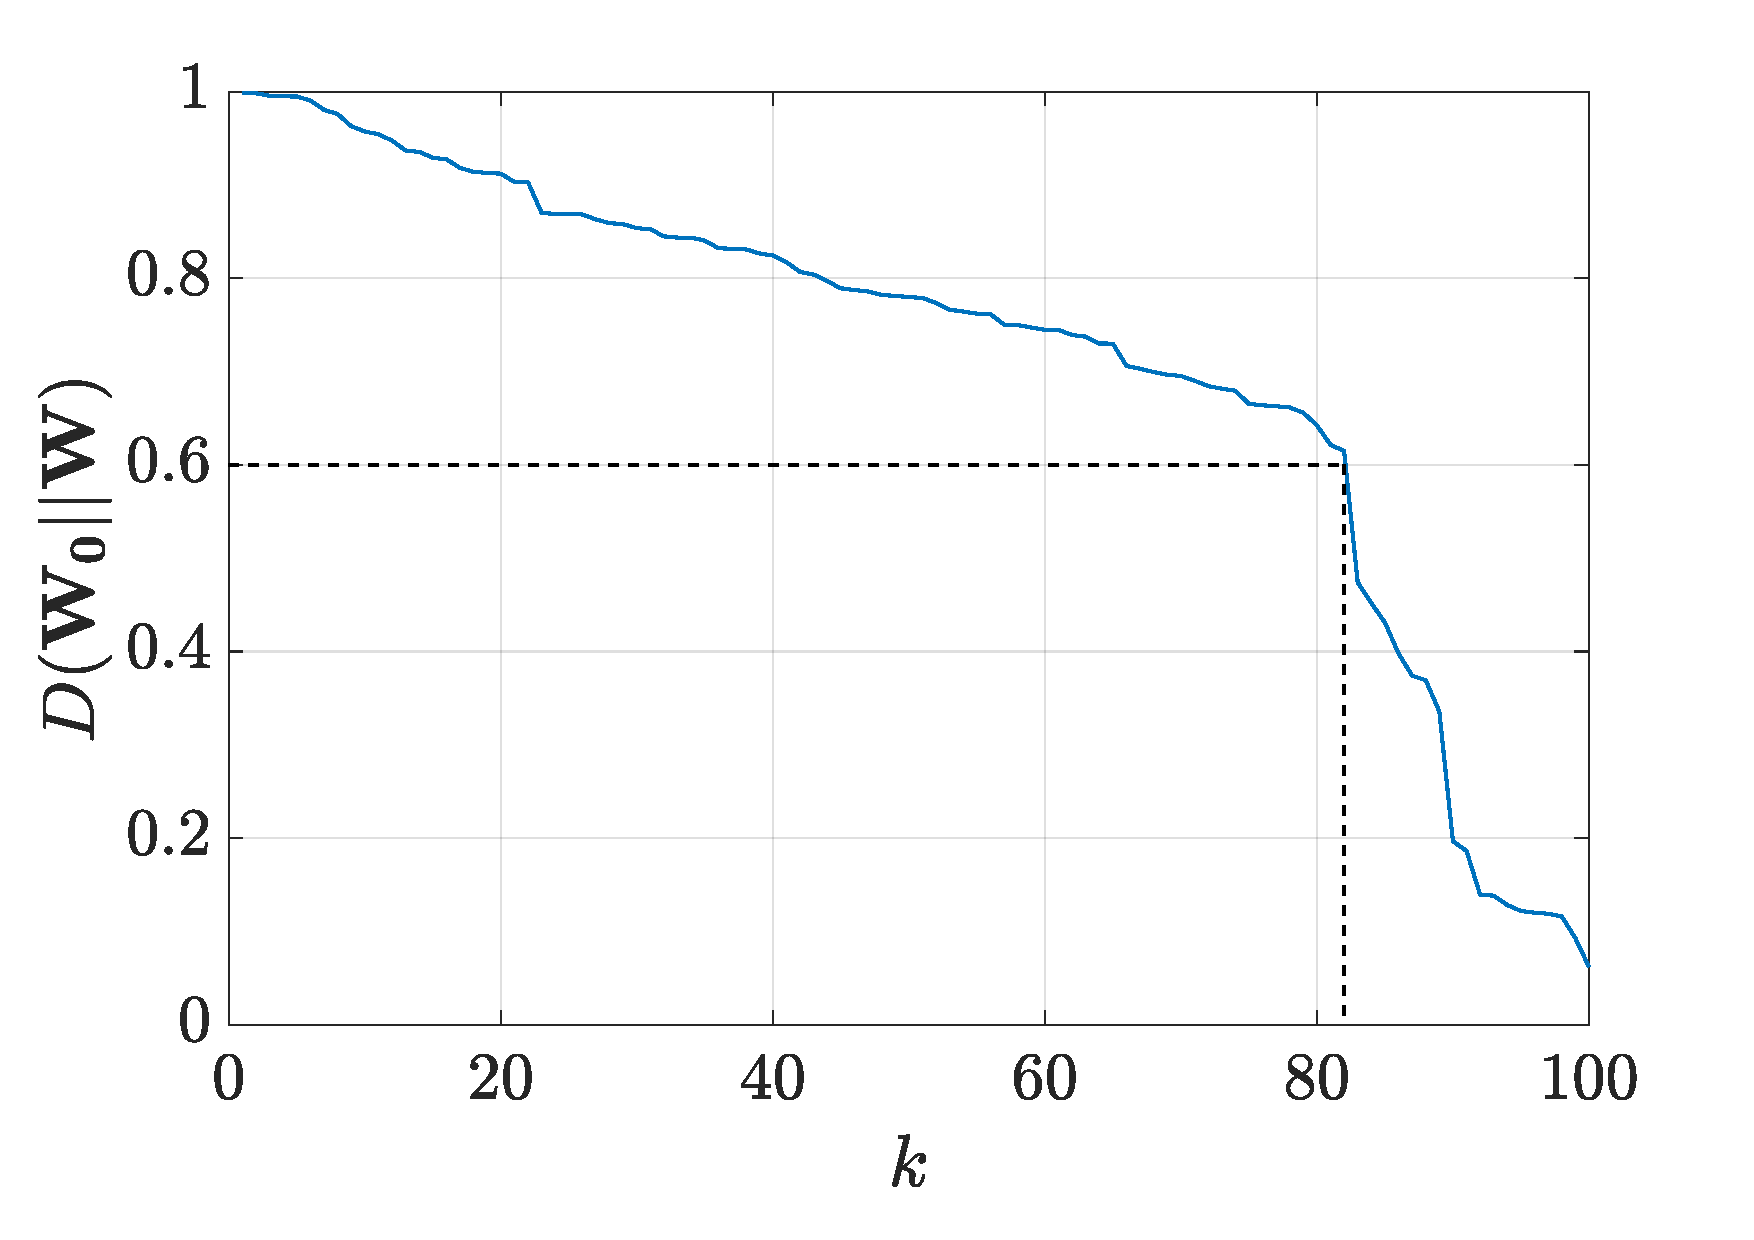
\includegraphics[width=0.8\linewidth]{figures/distanceCosLinDisplay.pdf}
\caption{Example of the $\mathbf{W}_{traffic}$ extraction from the sorted cosine similarity with a threshold $t = 0.6$. The $82$-nd first elements are considered as traffic component.}
\label{fig:W_TI_NMF}
\end{figure}

This approach is named \textit{Thresholded inititialized NMF} (TI-NMF). Other thresholding methods as the \textit{soft} \cite{donoho1995noising} and the \textit{firm} \cite{fornasier2008iterative} have been investigated. A fast parametric study revealed that the \textit{hard} thresholding method, as presented in  Figure \ref{fig:W_TI_NMF}, was the most reliable approach.

\section{Experimental protocol}\label{part:protocol}

In order to validate the usefulness of the proposed NMF scheme to estimate the road traffic noise levels, one need to compare the traffic noise level predicted by the algorithm to a reference level. The latter can hardly be measured or even annotated from real life recordings. Thus,  we propose to consider simulated sound scenes to assess the performance of the proposed NMF. This offers a controlled framework to design at low cost a wide diversity of sound environments in which all the traffic components are known, thus allowing the computation of the reference level. 

\subsection{Environmental sound scene corpus}

The corpus is designed with the \textit{SimScene} software\footnote{Open-source project available at: \url{https://bitbucket.org/mlagrange/simScene}}. \textit{SimScene} \cite{rossignol_simscene:_2015} is a simulator that creates monaural sound scenes in a .wav format by sequencing and summing audio samples that come from an isolated sound database. The simulator has been succesfully considered for a wide range of experimental design for sound detection algorithm assessment \cite{lafay:hal-01111381} \cite{benetos:hal-01520194} \cite{mesaros:hal-01650601}.

This database is divided into two categories: $i)$ the \textit{event} category, which are the brief sounds (from 1 to 20 seconds) that are considered as salient including 245 sound event samples divided in 19 sound classes (\textit{ringing bell, whistling bird, sweeping broom, car horn, passing car, hammer, drill, coughing, barking dog, rolling suitcase, closing door, plane, siren, footstep, storm, street noise, metallic noise, train, tramway, truck and voice}) and $ii)$ the \textit{background} or \textit{texture} category that includes all the sounds that are of long duration and whose acoustic properties do not vary with respect to time. 154 sound samples that belong to this category are divided in 9 sound classes (\textit{whistling bird, construction site noise, crowd noise, park, rain, children playing in schoolyard, constant traffic noise, ventilation, wind}). These sounds are in .wav format sampled at 44.1 kHz. The sound class \textit{car passages} comes from 60 recordings of 2 cars (Renault Megane and Renault Scenic) made on the Ifsttar's runway at different speeds with multiple gear ratio. The other audio files have been found online (\textit{freesound.org}) and within the \textit{UrbanSound8k} database \cite{salamon_dataset_nodate}. Each sound class is composed of multiples samples (\textit{bird01.wav}, \textit{bird02.wav} \dots) to allow some diversity in the resulting mixture.
The software allows the user to control some high level parameters (number of events of each class that appear in the mixture, elapsed time between each sample of a same class, presence of a fade in and a fade out \dots) completed with a standard deviation that may bring some random behavior between the scenes. Furthermore, an audio file of each sound class present in the scene can be generated that allows to know its exact contribution as well as a text file that summarizes the time presence of all the events.\\


\begin{figure}[t]
    \centering
    \begin{subfigure}[t]{0.47\linewidth}
        \centering
       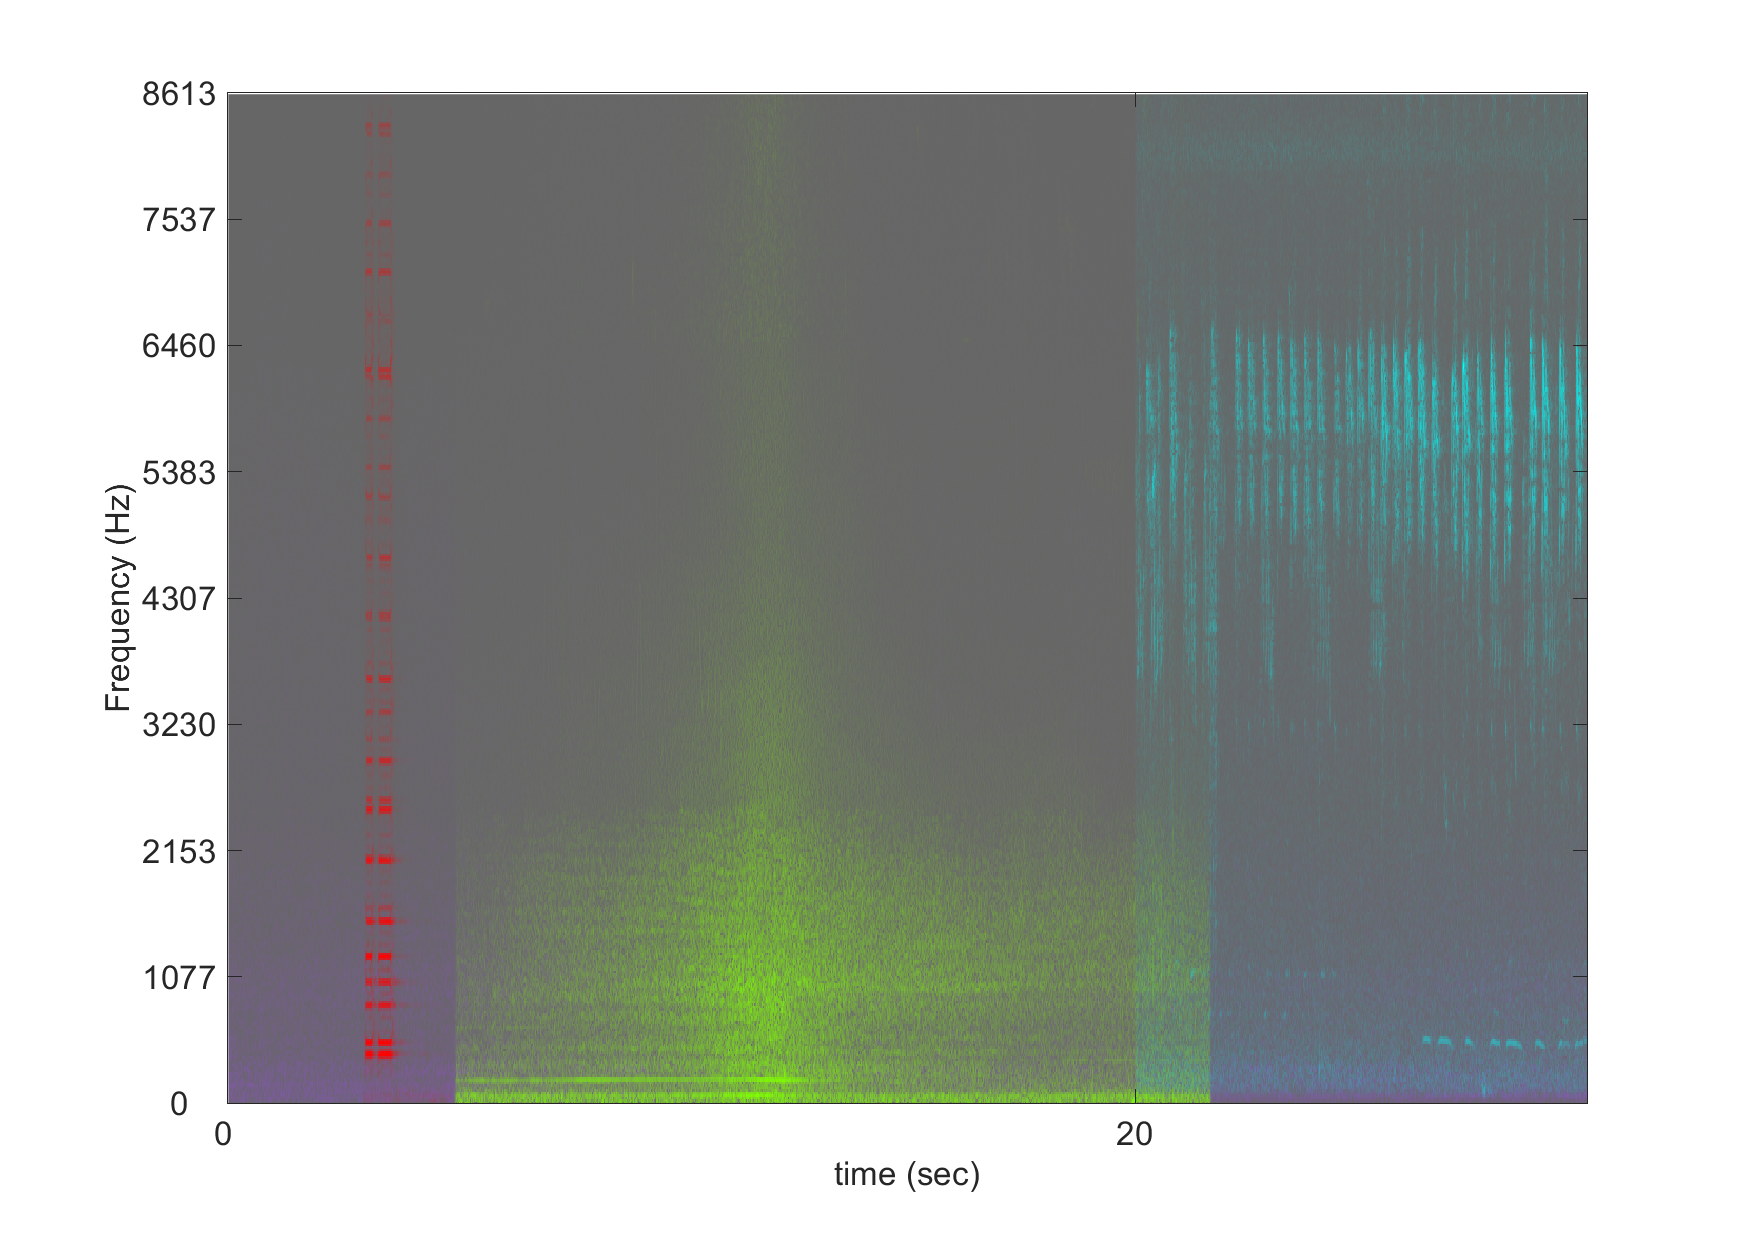
\includegraphics[width=\linewidth]{./figures/exempleSimScene3-spectrum.png}
       \caption{}
       \label{fig:simScene_spec}
    \end{subfigure}%
    \hfill
    \begin{subfigure}[t]{0.47\linewidth}
        \centering
       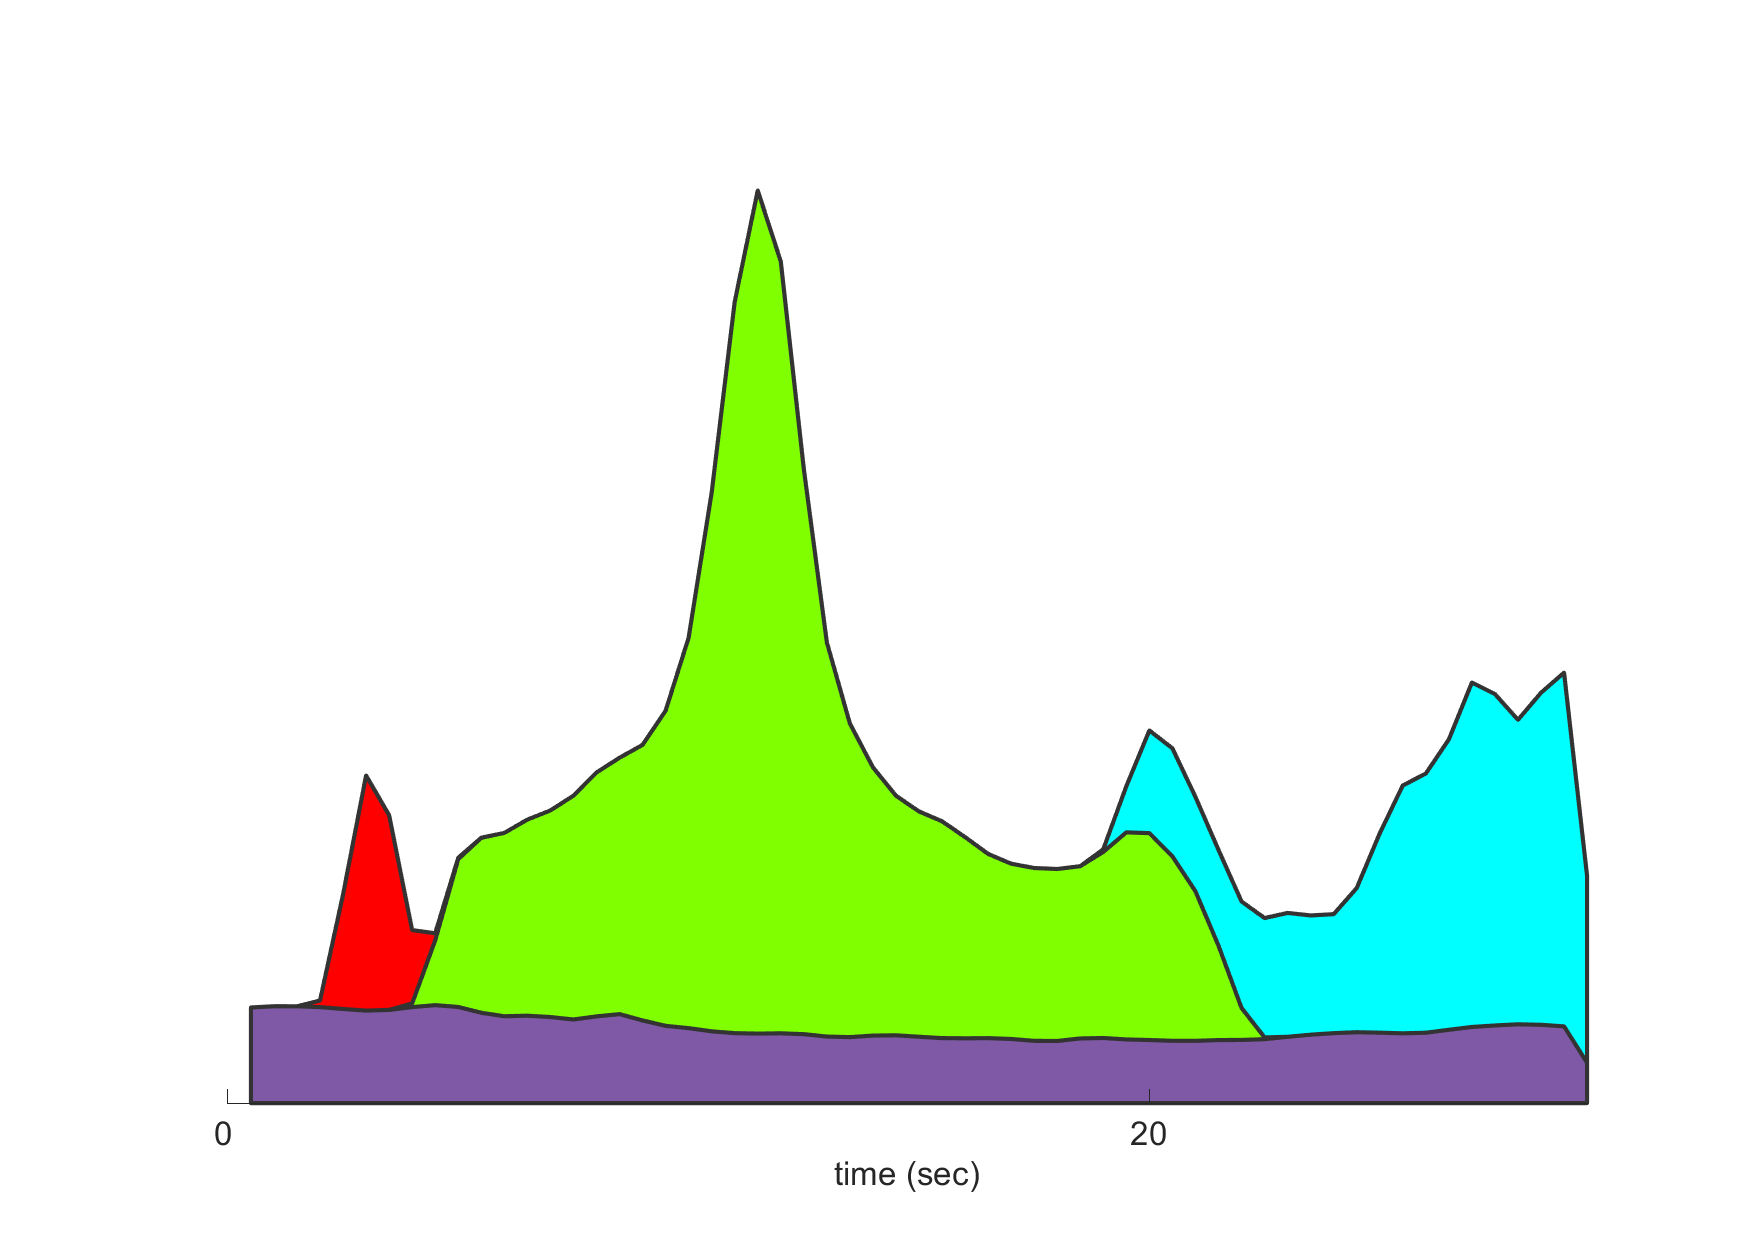
\includegraphics[width=\linewidth]{./figures/exempleSimScene3-timeDomain.png}
       \caption{}
       \label{fig:simScene_time}
    \end{subfigure}
    \caption{Example of a simple scene created with \textit{SimScene} software (the spectrogram (\subref{fig:simScene_spec}), the time domain \subref{fig:simScene_time})) with a sound background (road traffic in purple) and 3 sound events (car horn in red, car passage in green and whistling bird in blue)}
    \label{fig:example_simScene}
\end{figure}

This database allows us to create a wide diversity of realistic urban sound scenes from the road traffic point of view \cite{gloaguen_creation_2017}. A sound mixing corpus is composed of 6 sub-corpus of 25 audio files each lasting 30 seconds. Each sub-corpus is characterized by a specific generic sound class that summed with traffic will make the estimation of the traffic level more difficult. The classes are: \textit{alert} (car horn, siren), \textit{animals} (barking dog , whistling bird), \textit{climate} (wind, rain), \textit{humans} (crowd noise and voice), \textit{mechanics} (metallic and construction site noises) and \textit{transportation} (train, tramway and plane). In each file, traffic component is present as the sum of the background and event traffic sounds and is mixed with the other sound classes. The sound classes that are not related to the traffic component are summed up as the \textit{interfering} sound class. To test different scenarios, each audio file is duplicated with the traffic sound level of the entire sound scene, $L_{p,traffic}$, fixed to a specific level according to the sound level of the \textit{interfering} class, $L_{p,interfering}$,  following the relation (\ref{eq:tir}).

\begin{equation}\label{eq:tir}
TIR = L_{p,traffic}-L_{p,interfering}
\end{equation}

with the \textit{Traffic Interference Ratio} $TIR \in$ [-12 -6 0 6  12] dB. When $TIR < 0$ dB, the traffic component is then less present than the interfering class. In the opposite, for $TIR > 0$ dB, the traffic class is louder than the interfering class. The total number of scenes designed is 750 (6 sub-corpus $\times$ 25 scenes $\times$  5 $TIR$ values). The corpora are available for download at: \url{https://zenodo.org/record/1145855#.Wl2oPnkiGos}

\subsection{Experiment}

The experiment consists in estimating the road traffic sound level of the 6 environmental sound sub-corpus (\textit{alert} (al), \textit{animals} (an), \textit{humans} (hu), \textit{climate} (cl), \textit{mechanics} (me), \textit{transportation} (tr)) composed each of 25 audio files ($M$ = 25) and for 5 $TIR$ ([-12 -6 0 6 12] dB). The spectrogram $\mathbf{V}$ of each sound scene is built with a window size $w = 2^{12}$ with a 50 $\%$ overlap, see Figure \ref{fig:bloc_experiment}.

\begin{figure}
    \centering
    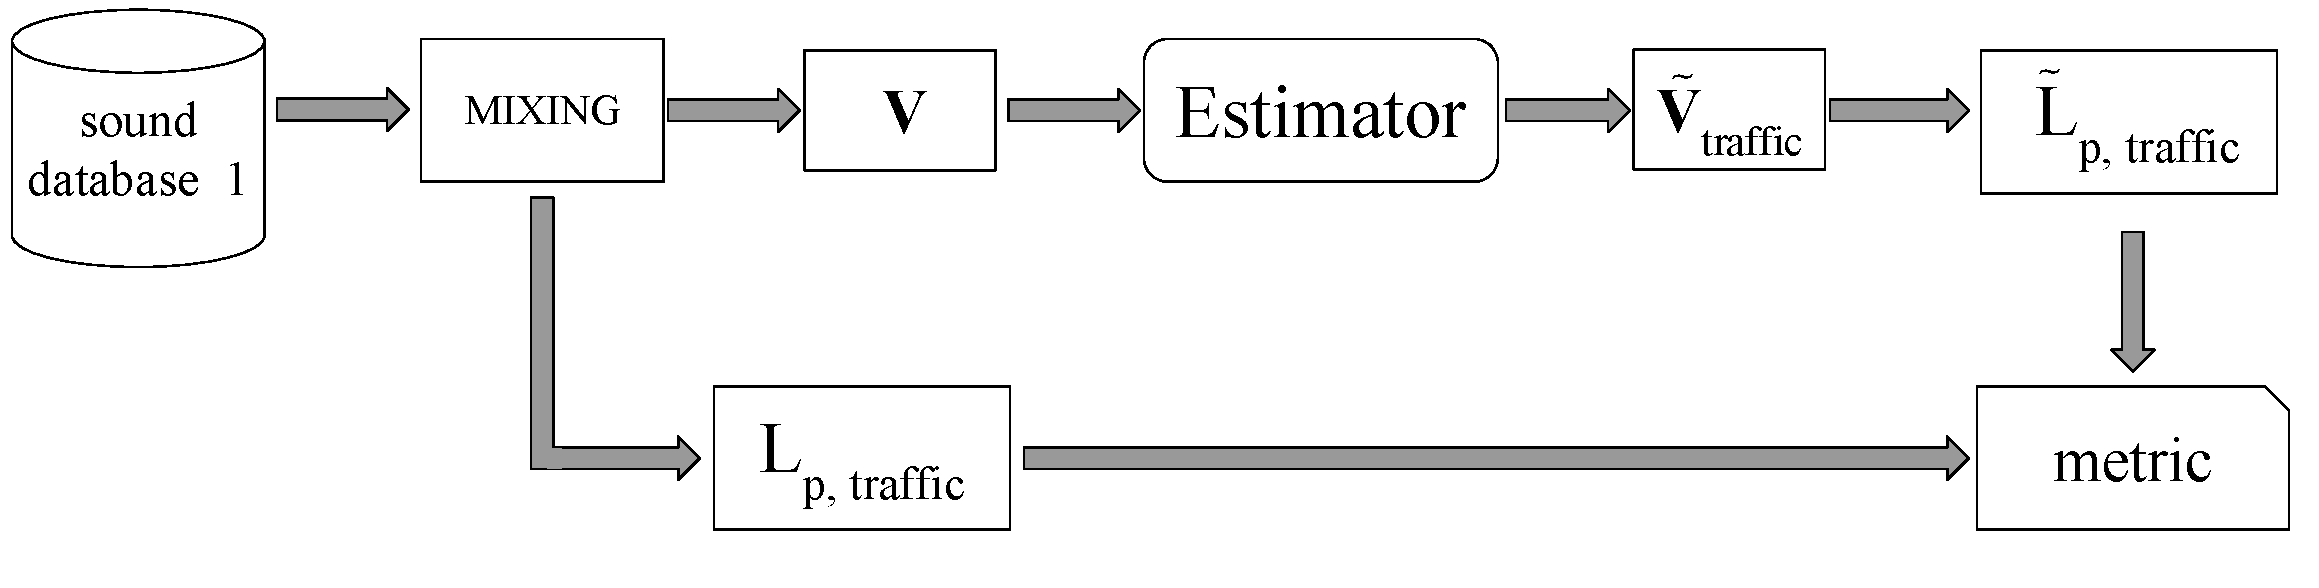
\includegraphics[width=\linewidth]{figures/bloc_diagram_estimator.pdf}
    \caption{Block diagram of the experience with the urban sound scenes sound mixture step and the estimation step. The estimator may be a frequency low-pass filter or NMF}
    \label{fig:bloc_experiment}
\end{figure}

Assuming that the traffic spectral profile is largely concentrated in the low frequency components, a first estimator to determine the traffic sound level is a frequency low-pass filter. It depends only on the cut-off frequencies $f_c \in $ [500 1k 2k 5k 10k 20k] Hz. The spectrogram $\mathbf{V}$ is filtered and the remaining energy is then considered as traffic component (eq. \ref{eq:v_tr_filtered}),

\begin{equation}\label{eq:v_tr_filtered}
\mathbf{\tilde{V}}_{traffic} = \mathbf{V}_{f_c}.
\end{equation}

The second estimator is the proposed scheme, based on the three NMF schemes presented in Section \ref{part:nmf}. Multiples experimental factors are involved here between the dictionary learning and NMF (see Figure \ref{fig:bloc_nmf}), each experimental factor having multiples modalities.

\begin{figure}
    \centering
    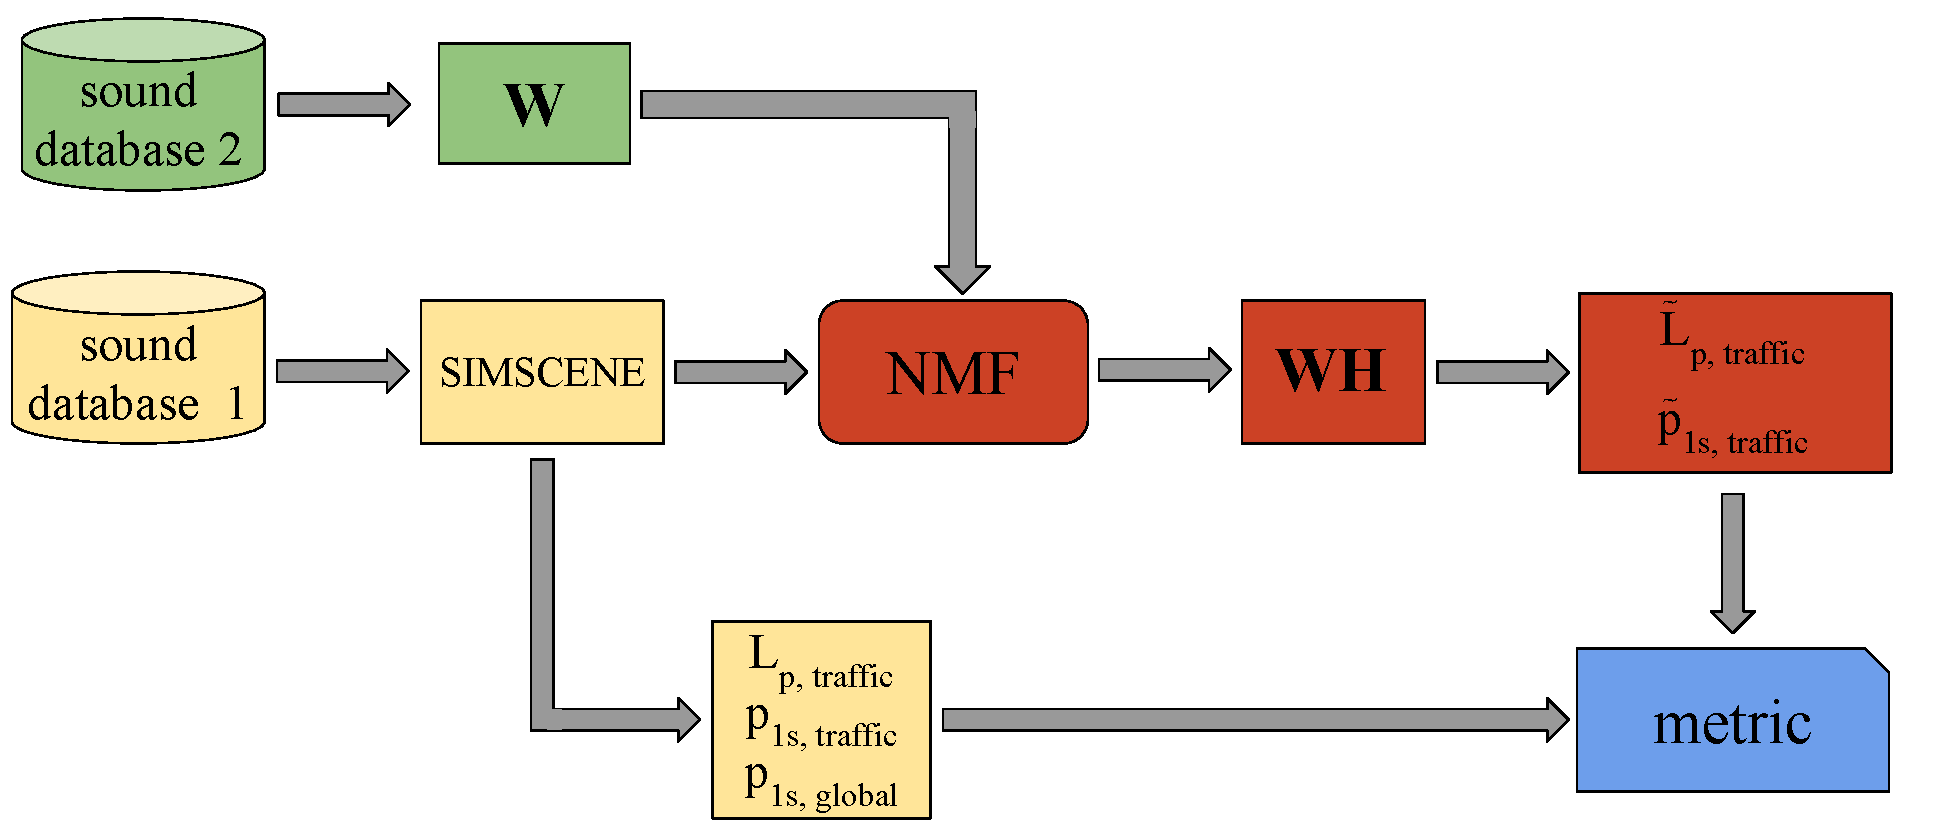
\includegraphics[width=\linewidth]{figures/bloc_diagram_NMF_EN.pdf}
    \caption{Block diagram of the NMF experience with the dictionary design composed from a second sound database}
    \label{fig:bloc_nmf}
\end{figure}

\begin{table*}[t]
\centering

\begin{tabularx}{17.5cm}{L{3cm}@{}C{12cm}@{}C{2cm}@{}}
	\hline
    \textbf{\begin{tabular}[c]{@{}l@{}}experimental \\ factors\end{tabular}} & modalities & \begin{tabular}[c]{@{}l@{}}number  \\ of level\end{tabular}\\ \toprule
\end{tabularx}

\begin{tabularx}{17.5cm}{L{3cm}@{}C{2cm}@{}C{2cm}@{}@{}C{2cm}@{}@{}C{2cm}@{}@{}C{2cm}@{}@{}C{2cm}@{}@{}C{2cm}@{}}
    \textbf{sub-classes} & alert & animals & climate & humans & transportation & mechanics  & 6
\end{tabularx}

\begin{tabularx}{17.5cm}{L{3cm}@{}C{2.4cm}@{}@{}C{2.4cm}@{}@{}C{2.4cm}@{}@{}C{2.4cm}@{}@{}C{2.4cm}@{}C{2cm}@{}}
\rowcolor[HTML]{C0C0C0} 
   $\mathbf{TIR}$ (dB) & -12 & -6 & 0 & 6 & 12 & 5\\
\end{tabularx}


\begin{tabularx}{17.5cm}{L{3cm}@{}C{2cm}@{}C{2cm}@{}@{}C{2cm}@{}@{}C{2cm}@{}@{}C{2cm}@{}@{}C{2cm}@{}@{}C{2cm}@{}}
   $\mathbf{f_c}$ (kHz) & 0.5 & 1 & 2 & 5 & 10 & 20  & 6\\
   \bottomrule
\end{tabularx}


\caption{Summary of the different experimental factors and their modalities taken into account in the frequency low-pass filter estimator}
\label{tab:experimental_factorsFilter}
\end{table*}


\begin{table*}[t]
\centering

\begin{tabularx}{17.5cm}{L{3cm}@{}C{12cm}@{}@{}C{2cm}}
	\hline
    \textbf{\begin{tabular}[c]{@{}l@{}}experimental \\ factors\end{tabular}} & modalities & \begin{tabular}[c]{@{}l@{}}number \\ of modality\end{tabular}\\ \toprule
\end{tabularx}

\begin{tabularx}{17.5cm}{L{3cm}@{}C{2cm}@{}C{2cm}@{}@{}C{2cm}@{}@{}C{2cm}@{}@{}C{2cm}@{}@{}C{2cm}@{}@{}C{2cm}@{}}
    \textbf{sub-classes} & alert & animals & climate & humans & transportation & mechanics & 6 
\end{tabularx}

\begin{tabularx}{17.5cm}{L{3cm}@{}C{2.4cm}@{}@{}C{2.4cm}@{}@{}C{2.4cm}@{}@{}C{2.4cm}@{}@{}C{2.4cm}@{}C{2cm}@{}}
\rowcolor[HTML]{C0C0C0} 
   $\mathbf{TIR}$ (dB) & -12 & -6 & 0 & 6 & 12 & 5 \\
\end{tabularx}

\begin{tabularx}{17.5cm}{L{3cm}@{}C{4cm}@{}@{}@{}C{4cm}@{}@{}C{4cm}@{}C{2cm}@{}}
  \textbf{method} & Sup-NMF & Sem-NMF & TI-NMF & 3 \\
\end{tabularx}

\begin{tabularx}{17.5cm}{L{3cm}@{}C{4cm}@{}@{}C{4cm}@{}@{}C{4cm}@{}C{2cm}@{}}
\rowcolor[HTML]{C0C0C0}
    $\mathbf{w_t}$ (s) & 0.5 & 1 & \textit{all} & 3 
\end{tabularx}

\begin{tabularx}{17.5cm}{L{3cm}@{}C{3cm}@{}@{}C{3cm}@{}@{}C{3cm}@{}@{}C{3cm}@{}C{2cm}@{}}
    $\mathbf{K}$ & 25 & 50 & 100 & 200  & 4\\
\end{tabularx}


\begin{tabularx}{17.5cm}{L{3cm}@{}C{6cm}@{}@{}C{6cm}@{}C{2cm}@{}}
\rowcolor[HTML]{C0C0C0}
   $\mathbf{\beta}$ & 1 & 2 & 2\\
\end{tabularx}

\begin{tabularx}{17.5cm}{L{3cm}@{}C{12cm}@{}C{2cm}@{}}
   $\mathbf{t}$  &  from 0.30 to 0.70 with 0.01 step & 40\\
   \bottomrule
\end{tabularx}
\caption{Summary of the different experimental factors and their modalities taken into account in NMF estimator}
\label{tab:experimental_factorsNMF}
\end{table*}


\subsubsection{NMF Dictionary}\label{part:dictionary_learning}

In order to prevent potential overfitting issues, the dictionary is built from a separate sound database dedicated specifically to this task. It is composed of 53 audio files of passing cars. These recordings have been made on the Ifsttar's runway too, with the same experimental conditions that the recordings of the \textit{SimScene} database but with two different cars (Dacia Sandero and Renault Clio). First, for each audio file, its spectrogram is calculated with fixed parameters ($w$, 50 $\%$ overlap, $nfft$). Then time/frequency windows of $F \times w_t $ dimensions are applied without overlapping on the spectrogram in order to consider several spectra for each audio file where $w_t \in [0.5~1]$ second. In each window, the root mean square value is calculated on each frequency bin to reduce the windowed spectrogram in one spectrum a of $F \times 1$ dimension. With this size of window, it is possible to obtain the characteristic pitches of the different audio samples. One obtain for each value of $w_t$, from the 53 audio samples of passing cars respectively 2218 and 1109 elements. Since the number of elements given by this processing is high, in order to reduce the computational time and avoid redundant information, a $K$-means clustering is applied to reduce the number of spectra to $K \in \left[ 25, 50, 100, 200\right]$. The $K$ centroids are then the elements of the dictionary. A special case is added where the root mean square of \textit{all} the spectrogram is applied ($w_t$ = $all$) in order to build a dictionary with the spectral envelope of each audio sample. In this case, 53 spectra are obtained. The $K$-means clustering algorithm is then reduced to $K \in \left[25 50 \right]$.

\begin{figure}[t!]
    \centering
    \begin{subfigure}[t]{0.47\linewidth}
        \centering
       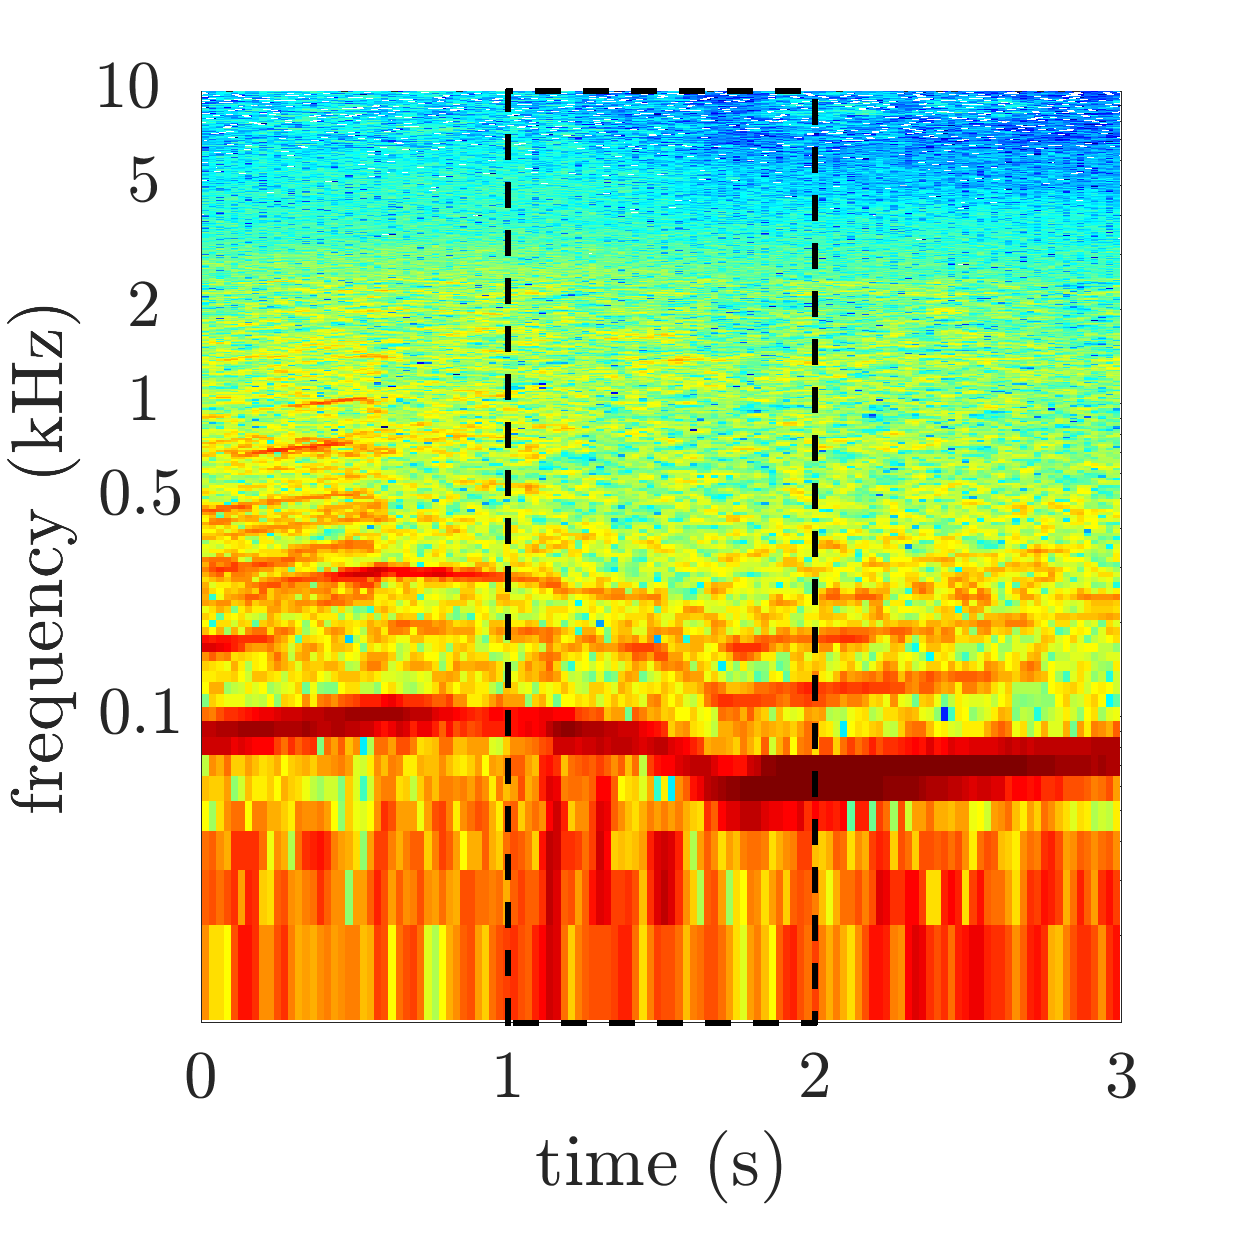
\includegraphics[height=4.5cm]{figures/dictionary3.pdf}
       \caption{}
        \label{fig:specW}
    \end{subfigure}%
    \hfill
    \begin{subfigure}[t]{0.47\linewidth}
        \centering
       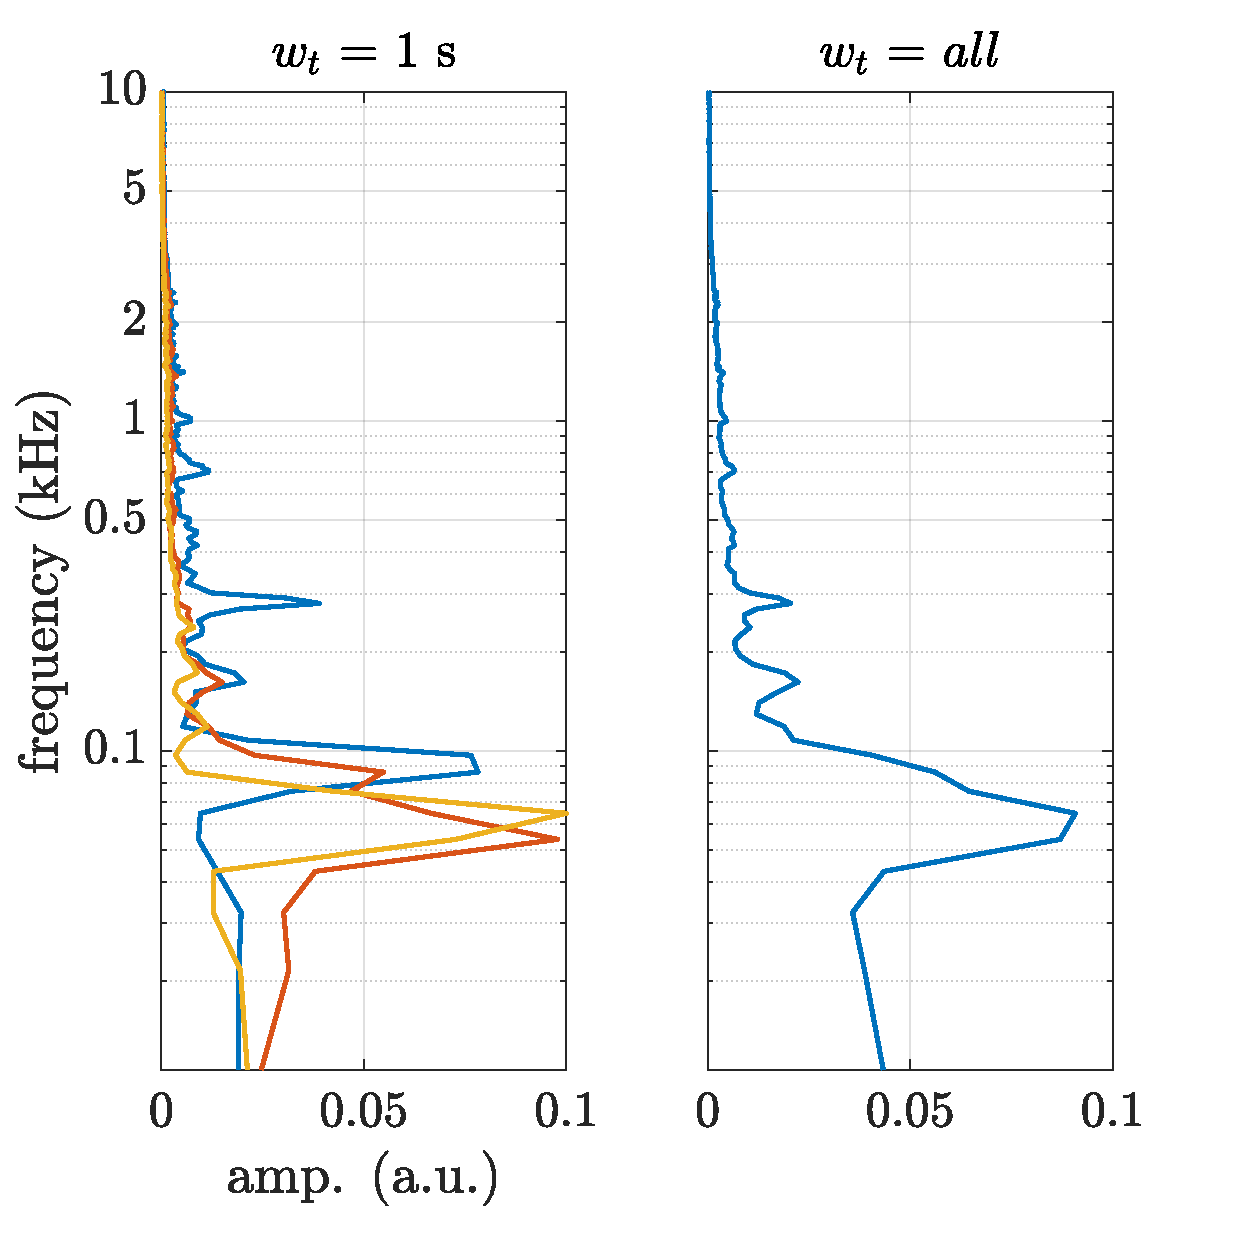
\includegraphics[height=4.5cm]{figures/dictionary4.pdf}
        \caption{}
        \label{fig:ElementW}
    \end{subfigure}
    \caption{Example of the dictionary building with a 3 second extract of a car passage. In dashed lines, a 1 second $w_t$ window  (\subref{fig:specW}). With $w_t$ = 1 second, 3 spectra are then generated and included in $\mathbf{W}$ while for $w_t$ = $all$, the audio file is reduced into 1 spectral vector (\subref{fig:ElementW})}
    \label{fig:spec_elementW}
\end{figure}


An example that illustrates the process can be found on Figure \ref{fig:spec_elementW} on a 3 second extract of the spectrogram of a car passage, see Figure \ref{fig:specW}. In the case where $w_t$ = 1 second, 3 elements are therefore extracted from the spectrogram while in the case where $w_t$ = \textit{all}, all the spectrogram is reduced into one element, see Figure \ref{fig:ElementW}.

The obtained dictionary is expressed with third octave bands and each basis vector of $\mathbf{W}$ is normalized such as $\vert \vert \mathbf{W_k} \vert \vert = 1$ with $\vert \vert \bullet \vert\vert$ the $\ell$-1 norm. Table \ref{tab:experimental_factorsNMF} summarizes the experimental factors ($K$ and $w_t$) for the dictionary building and their related modalities. This last step allows us to reduce the dimensionality while preserving a rich description of the spectral content. Experimental validation consistently showed that considering octave bands do not impact the performance for the two estimators studied in this paper.

\subsubsection{Experimental factors of NMF}

Sup-NMF and Sem-NMF updates are computed for 400 iterations, which is sufficient to reach convergence. TI-NMF is performed on a lower number of iterations (60) to prevent $\mathbf{W}$ to not deviate too much from the initial dictionary.
%\ml{ca c'est pas genial, il aurait mieux vallu utiliser un coefficient de pondération pour que W n'avance pas trop vite...}

The spectrogram $\mathbf{V}$ and the dictionary $\mathbf{W}$ are expressed with third octave bands ($F$ = 29). This coarser method allows the reduction of the matrix size and decreases the computation time. But,  must of all, by expressing the frequency axis on a log frequency axis,  the low frequencies, where the traffic energy is focused, are described more finely than the high frequencies. For TI-NMF, the threshold $t$ is set between 0.30 and 0.70 with a step of 0.01. Tables  \ref{tab:experimental_factorsFilter} and \ref{tab:experimental_factorsNMF} summarize the experimental factors and their related modalities. 

Considering the experimental settings derived from the different modalities of each experimental factor described in Table \ref{tab:experimental_factorsFilter}  between the 5 levels of $TIR$, the 6 sub-classes and the 6 cut-off frequencies $f_c$, 180 settings are performed. For Sup-NMF and Sem-NMF, according to Table \ref{tab:experimental_factorsNMF},  1200 associations of factors are made where the 4 levels of $K$ are associated with $w_t \in$ [0.5 1] s whereas only 2 levels of $K$ (25 and 50) are associated with $w_t = all$, see part \ref{part:dictionary_learning}. For TI-NMF, 24000 combinations are computed. In all, 25380 settings are performed between the different forms of the dictionary $\mathbf{W}$ and the multiple experimental factors

After having performed NMF on one scene, the average traffic sound level, $\tilde{L}_{p,traffic}$, of the entire scene is calculated, 

\begin{equation}
\tilde{L}_{p,traffic} = 20\log_{10}\left(\frac{p_{rms}}{p_0}\right)
\end{equation}

where $p_{rms}$ is the effective pressure deducted from $\left[\mathbf{WH} \right]_{traffic}$ and $p_0$ is the reference sound pressure, $p_0 = 2 \times 10^{-5} Pa$.  For each set of unique modalities of experimental factors, $M$ values of $\tilde{L}_{p,traffic}$, corresponding to the $M$ scenes, are then obtained. 


\begin{table*}[t]
\centering
\begin{tabular}{@{}ccccccc@{}}
\toprule
\textbf{method} & $f_c$ (kHz) & $\mathbf{\beta}$ & $\mathbf{K}$ & $\mathbf{w_t}$ (s) &   $\mathbf{t}$ & \textbf{$MAE$ (dB)} \\ \midrule
filter & 20  &  &  &  &  & 4.69 ($\pm$ 4.52) \\
filter & 0.5 &  &  &  &  & 2.89 ($\pm$ 2.84) \\ \hline \hline
Sup-NMF &  & 1 & 50 & 0.5  &  & 3.44 ($\pm$ 3.70) \\
Sup-NMF &  & 2 & 50 & 0.5  &  & 3.02 ($\pm$ 3.33) \\ \hline \hline
Sem-NMF &  & 1 & 100 & 0.5 &   & 2.33 ($\pm$ 1.10) \\
Sem-NMF &  & 2 & 100 & 0.5 &   & 2.32 ($\pm$ 1.26) \\ \hline \hline
\textbf{TI-NMF} &  & \textbf{1} & \textbf{200} & \textbf{0.5} &  \textbf{0.42} &\textbf{2.19 ($\pm$ 2.18)} \\
TI-NMF &  & 2 & 25 & all &  0.54 & 2.20 ($\pm$ 2.26)\\ \bottomrule
\end{tabular}
\caption{Best results for all the scenes according to the experimental factors $\beta$ and \textit{method} (in bold letter, the lowest error).}
\label{tab:results}
\end{table*}

\begin{table*}[t]
\centering
\begin{tabular}{@{}cccccc@{}}
\toprule
\textbf{method} & filter & filter & Sup-NMF & Sem-NMF & TI-NMF \\ \midrule
$f_c$ (kHz) & 20 & 0.5 &  &  &  \\
$\mathbf{\beta}$ &  &  & 2 & 2 & 1 \\ \hline
\textbf{-12} & 12.25 ($\pm$ 0.05) & 7.36 ($\pm$ 3.00) & 8.65 ($\pm$ 1.88) & 3.88 ($\pm$ 1.52) & 5.35 ($\pm$ 2.71) \\
\textbf{-6} & 6.96 ($\pm$ 0.05) & 3.44 ($\pm$ 1.65) & 4.22 ($\pm$ 1.27) & 1.37 ($\pm$ 0.71)  & 2.82 ($\pm$ 1.30) \\
\textbf{0} & 3.00 ($\pm$ 0.03) & 1.17 ($\pm$ 0.24) & 1.34 ($\pm$ 0.56) & 1.11 ($\pm$ 0.25) & 1.26 ($\pm$ 0.35) \\
\textbf{6} & 0.25 ($\pm$ 0.06) & 1.03 ($\pm$ 0.26) & 0.26 ($\pm$ 0.10) & 2.25 ($\pm$ 0.19) & 0.70 ($\pm$ 0.32) \\
\textbf{12} & 0.26 ($\pm$ 0.00) & 1.45 ($\pm$ 0.13) & 0.64 ($\pm$ 0.06) & 2.96 ($\pm$ 0.21)  & 0.84 ($\pm$ 0.24) \\ \bottomrule
\end{tabular}
\caption{$MAE$ error averaged on all sub-classes on each $TIR$ for the best scenario according to each method}
\label{tab:results_TIR}
\end{table*}


\subsubsection{Metrics}

The performance of the road traffic sound level estimator is assessed through the calculation of one reference metric, the Mean Absolute Error ($MAE$) \cite{willmott2005advantages}. It expresses the quality of the long-term reconstruction of the signal and consists in the average over the $M$ sound scenes of the absolute difference between the exact and estimated traffic sound level in dB,

\begin{equation}
MAE = \frac{\sum_{m = 1}^M\vert L^m_{p,traffic}-\tilde{L}^m_{p,traffic} \vert}{M}.
\end{equation}

\section{Results}\label{part:results}

Table \ref{tab:results} summarizes, according to the 2 main factors (\textit{method}, $\beta$), the lowest $MAE$ error averaged on all sub-classes and all $TIR$ (750 sound mixtures in all). For the low-pass frequency filters and each NMF approaches, the best parameter combinations are detailed according to the $TIR$ in Table \ref{tab:results_TIR},  and are expanded to the sub-classes in Figures \ref{fig:TIR_class_filter}, \ref{fig:TIR_class_sup}, \ref{fig:TIR_class_semi} and \ref{fig:TIR_class_TI}. \\

First, the errors produced by the filter are detailed. $f_c = 20 $ kHz is equivalent to consider all the sound mixtures without distinction between traffic and others sound sources. Consequently, in low $TIR$ (-12 dB and -6 dB), where traffic component is scarce, the error is more important than in high $TIR$ (6 dB and 12 dB) where the traffic component is predominant. $f_c = 500$ Hz is the cut-off frequency with the lowest mean error obtained. It is then considered as the baseline to compare the performances of NMF.

In low $TIR$, for \textit{alert} and \textit{animals}, which are sub-classes composed of higher frequencies, this filter is efficient as it removes these frequency components. For the other sub-classes where low frequency contents are present (storm for \textit{climate}, voices in \textit{humans}, planes, tramway and train in \textit{transport} and ventilation noise in \textit{mechanics}), the filter considers all the energy located in the pass-band and then does not dissociate the traffic element from the other sound sources. The errors are then nearly all superior to 4 dB and are overestimated, see Figure \ref{fig:alert_-12}. In opposite, in high $TIR$, the error is due to the energy removed from the traffic which has the consequence to underestimate the sound levels, see Figure \ref{fig:alert_12}. The 500 Hz filter finds a balance between what is put aside in low $TIR$ and what it is remained in high $TIR$. \\

\begin{figure*}[t]
    \centering
    \begin{subfigure}[t]{0.45\textwidth}
        \centering
        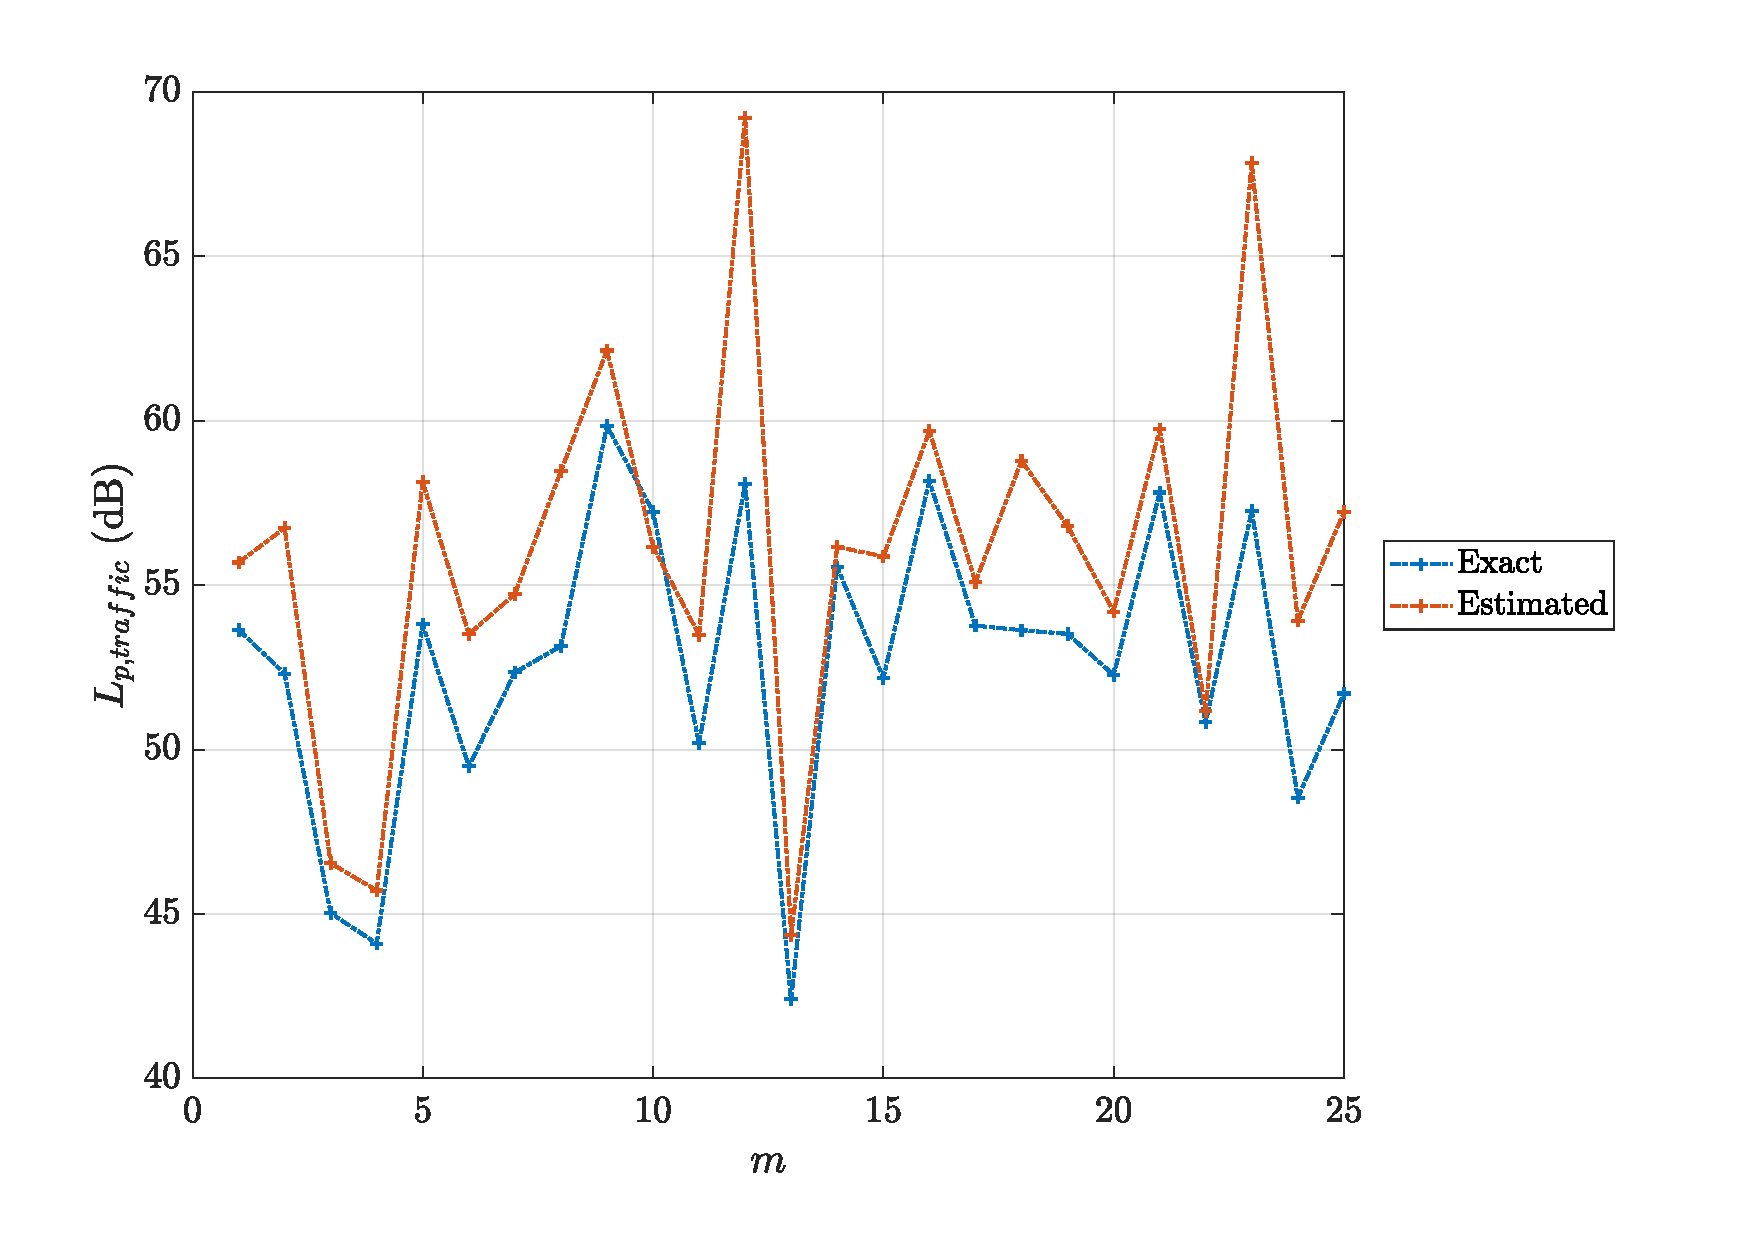
\includegraphics[width=\linewidth]{figures/LeqTrafficComparison_filter_alert_-12.pdf}
        \caption{}
        \label{fig:alert_-12}
    \end{subfigure}%
    \hfill
    \begin{subfigure}[t]{0.45\textwidth}
        \centering
        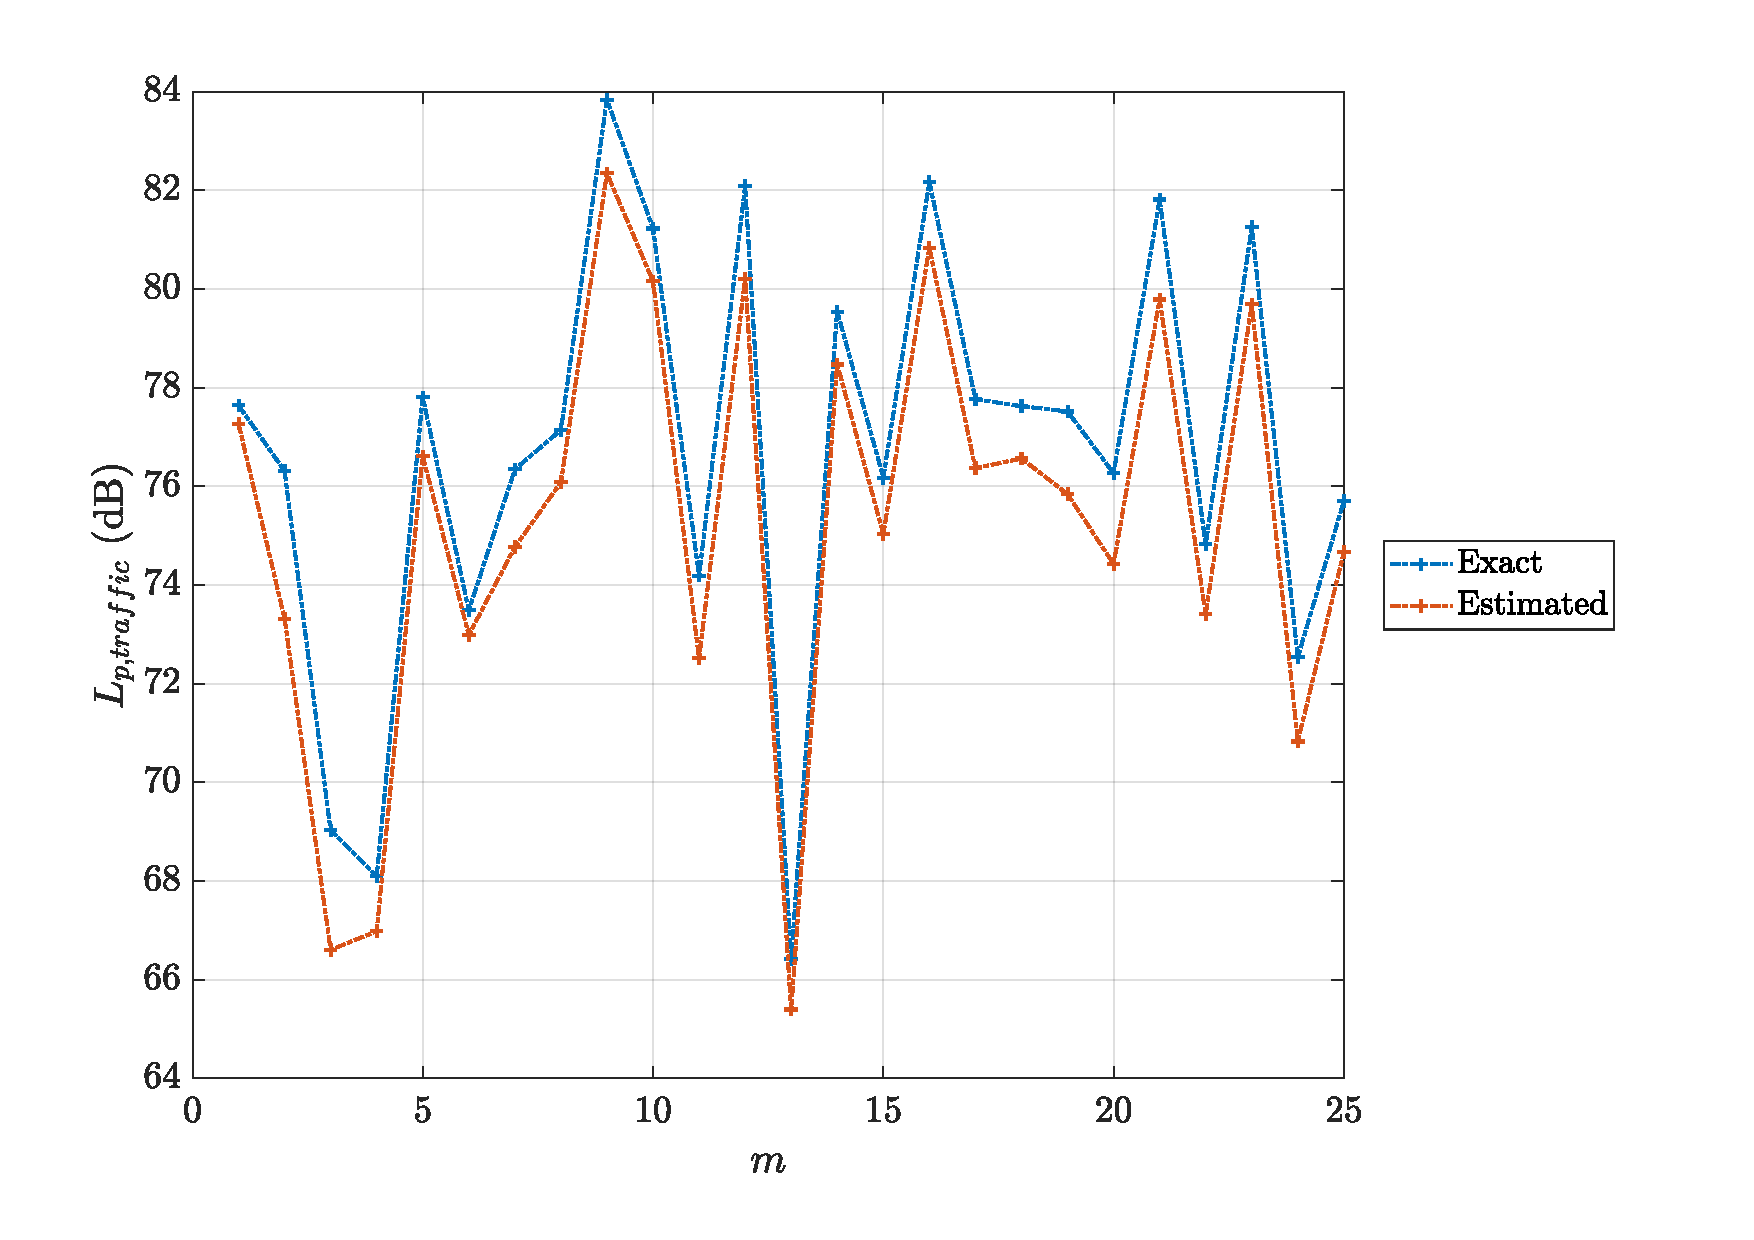
\includegraphics[width=\linewidth]{figures/LeqTrafficComparison_filter_alert_12.pdf}
        \caption{}
        \label{fig:alert_12}
    \end{subfigure}

    \caption{Global sound levels of the traffic estimated by the frequency low-pass filter with $f_c$ = 500 Hz for the M scenes of the sub-classes \textit{alert} at $TIR = -12$ dB(\subref{fig:alert_-12}) and at $TIR$ = 12 dB (\subref{fig:alert_12})}
    \label{fig:dictionaryExtraction}
\end{figure*}

Compared with the filter errors, the choice of some NMF approaches makes it possible to decrease the error of the road traffic sound level estimation. The supervised approach is the only method that has an average error superior to the 500 Hz filter baseline. Sem-NMF and TI-NMF have better results. The lowest average error is obtained for TI-NMF, 2.19 $\pm$ 2.18, for $\beta$ = 1 and threshold $t$ = 0.42 with the dictionary factors $K$ = 200 and $w_t$ = 500 ms. On the other hand, the semi-supervised approach has a higher error but with a lower standard deviation (2.32 $\pm$ 1.26).

\begin{figure*}[t]
    \centering
    \begin{subfigure}[t]{0.45\textwidth}
        \centering
        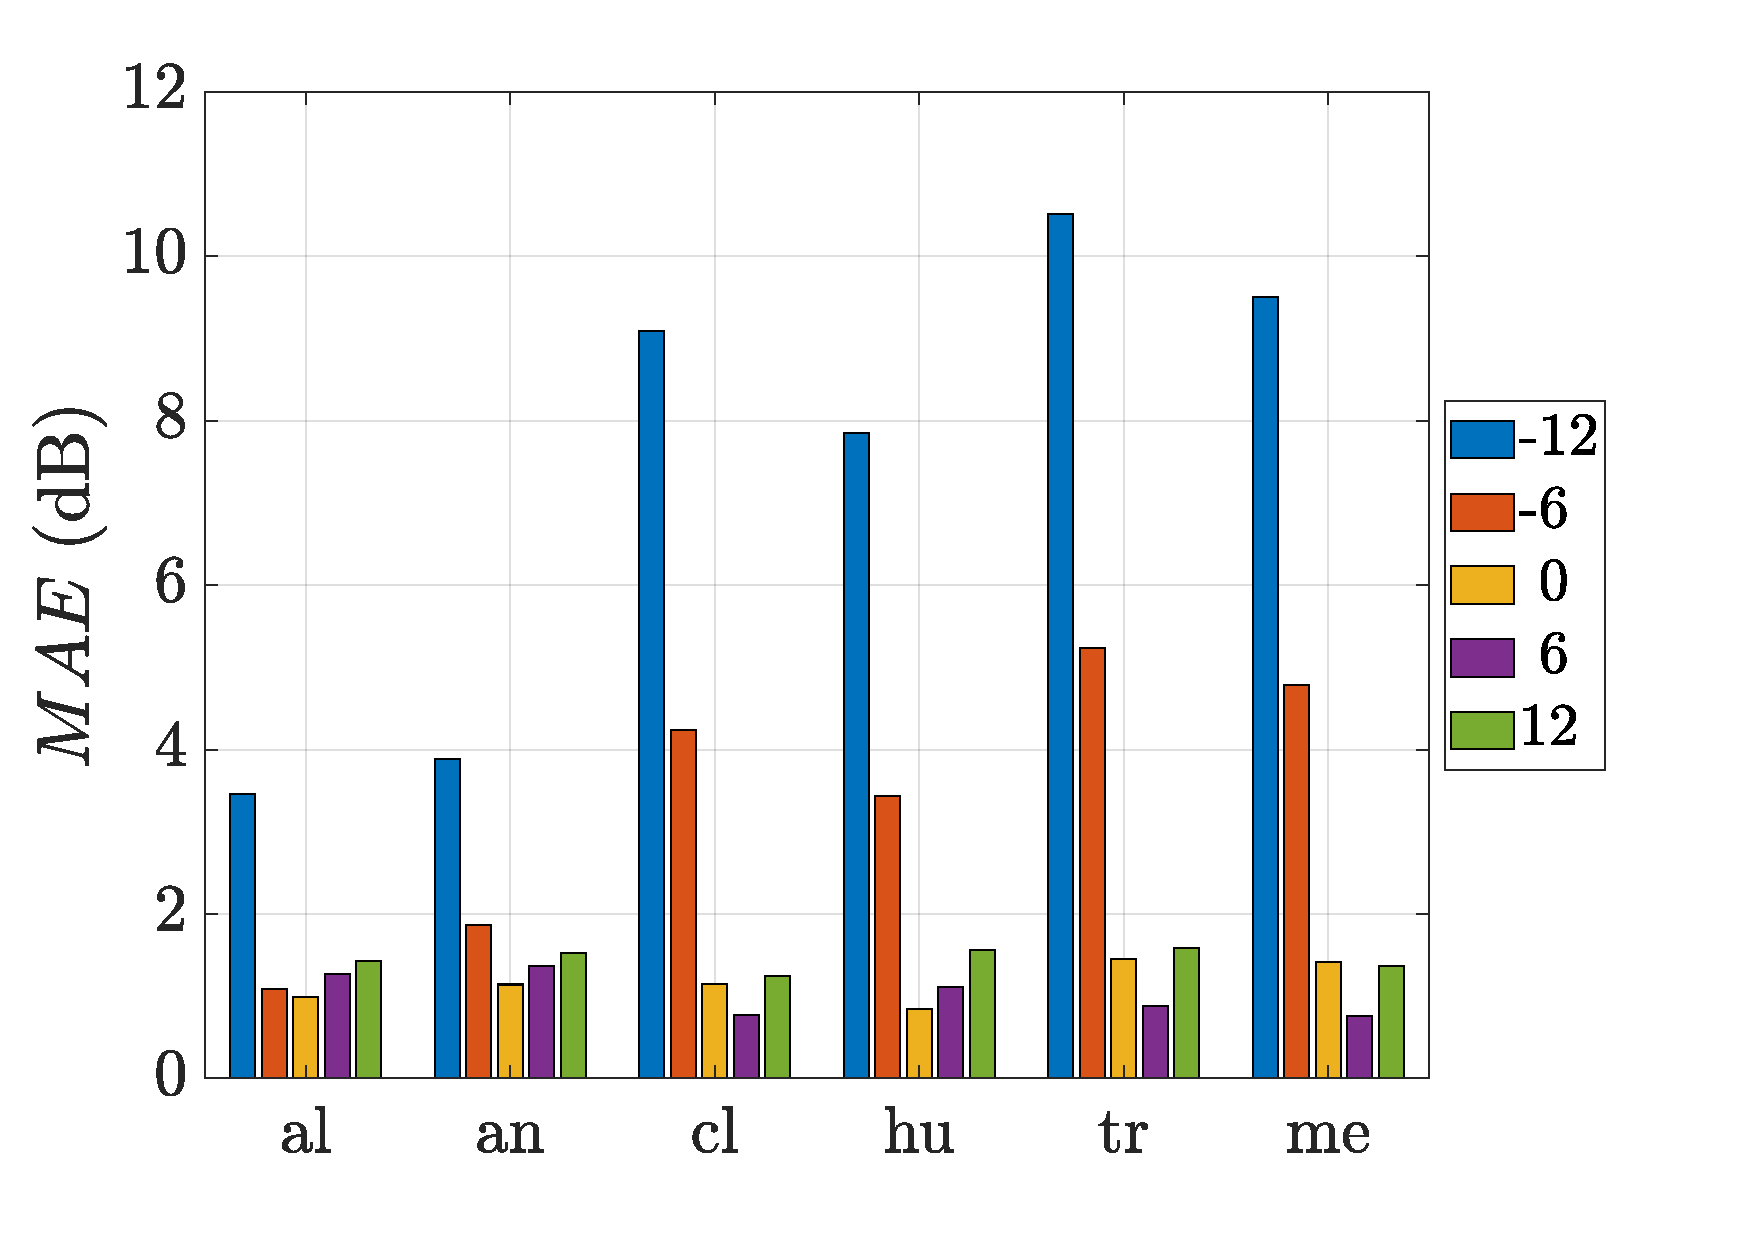
\includegraphics[width=\linewidth]{figures/filter_bar.pdf}
        \caption{Frequency low-pass filter with $f_c$ = 500 Hz}
        \label{fig:TIR_class_filter}
    \end{subfigure}%
    \hfill
    \begin{subfigure}[t]{0.45\textwidth}
        \centering
        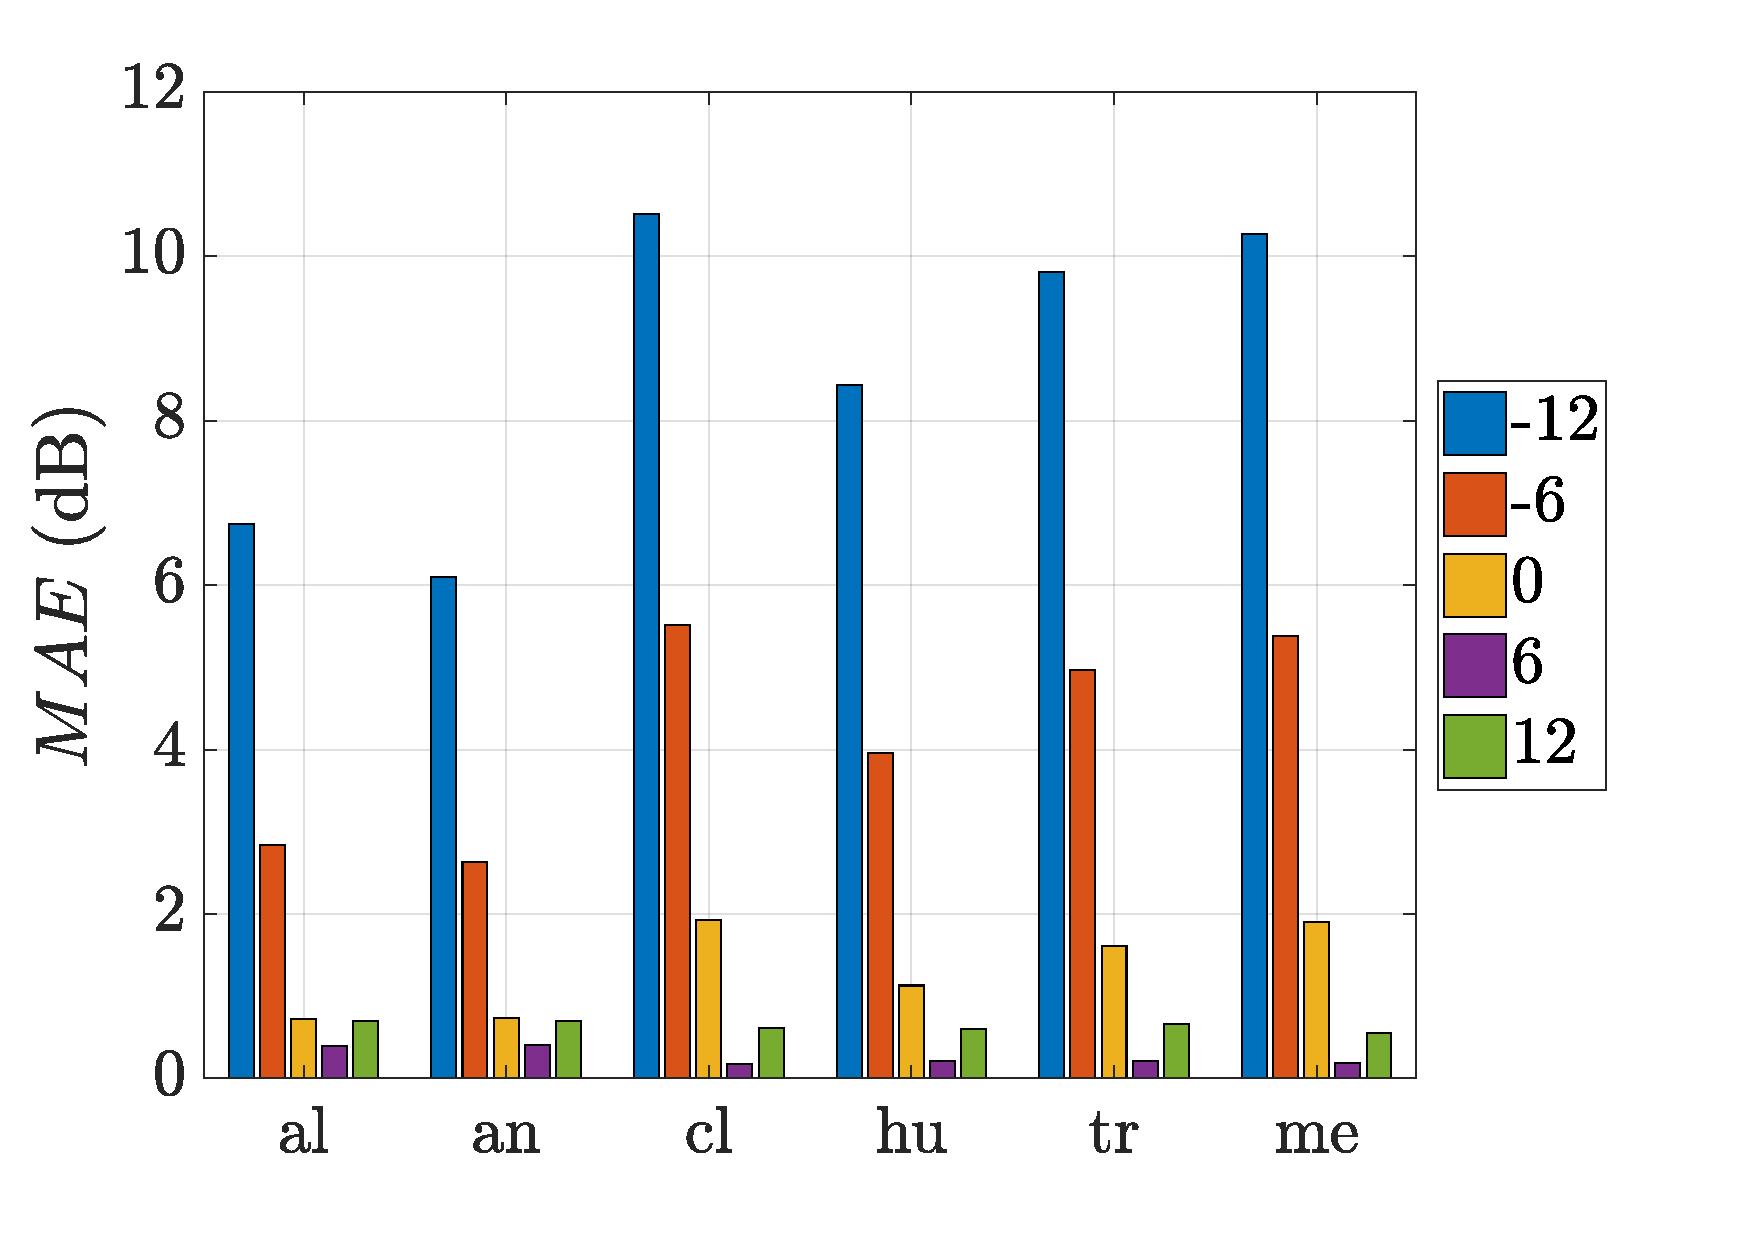
\includegraphics[width=\linewidth]{figures/sup_bar.pdf}
        \caption{$MAE$ error for each $TIR$ and sub-class with Sup-NMF and $\beta$ = 2}
                \label{fig:TIR_class_sup}
    \end{subfigure}

    \begin{subfigure}[t]{0.45\textwidth}
        \centering
      	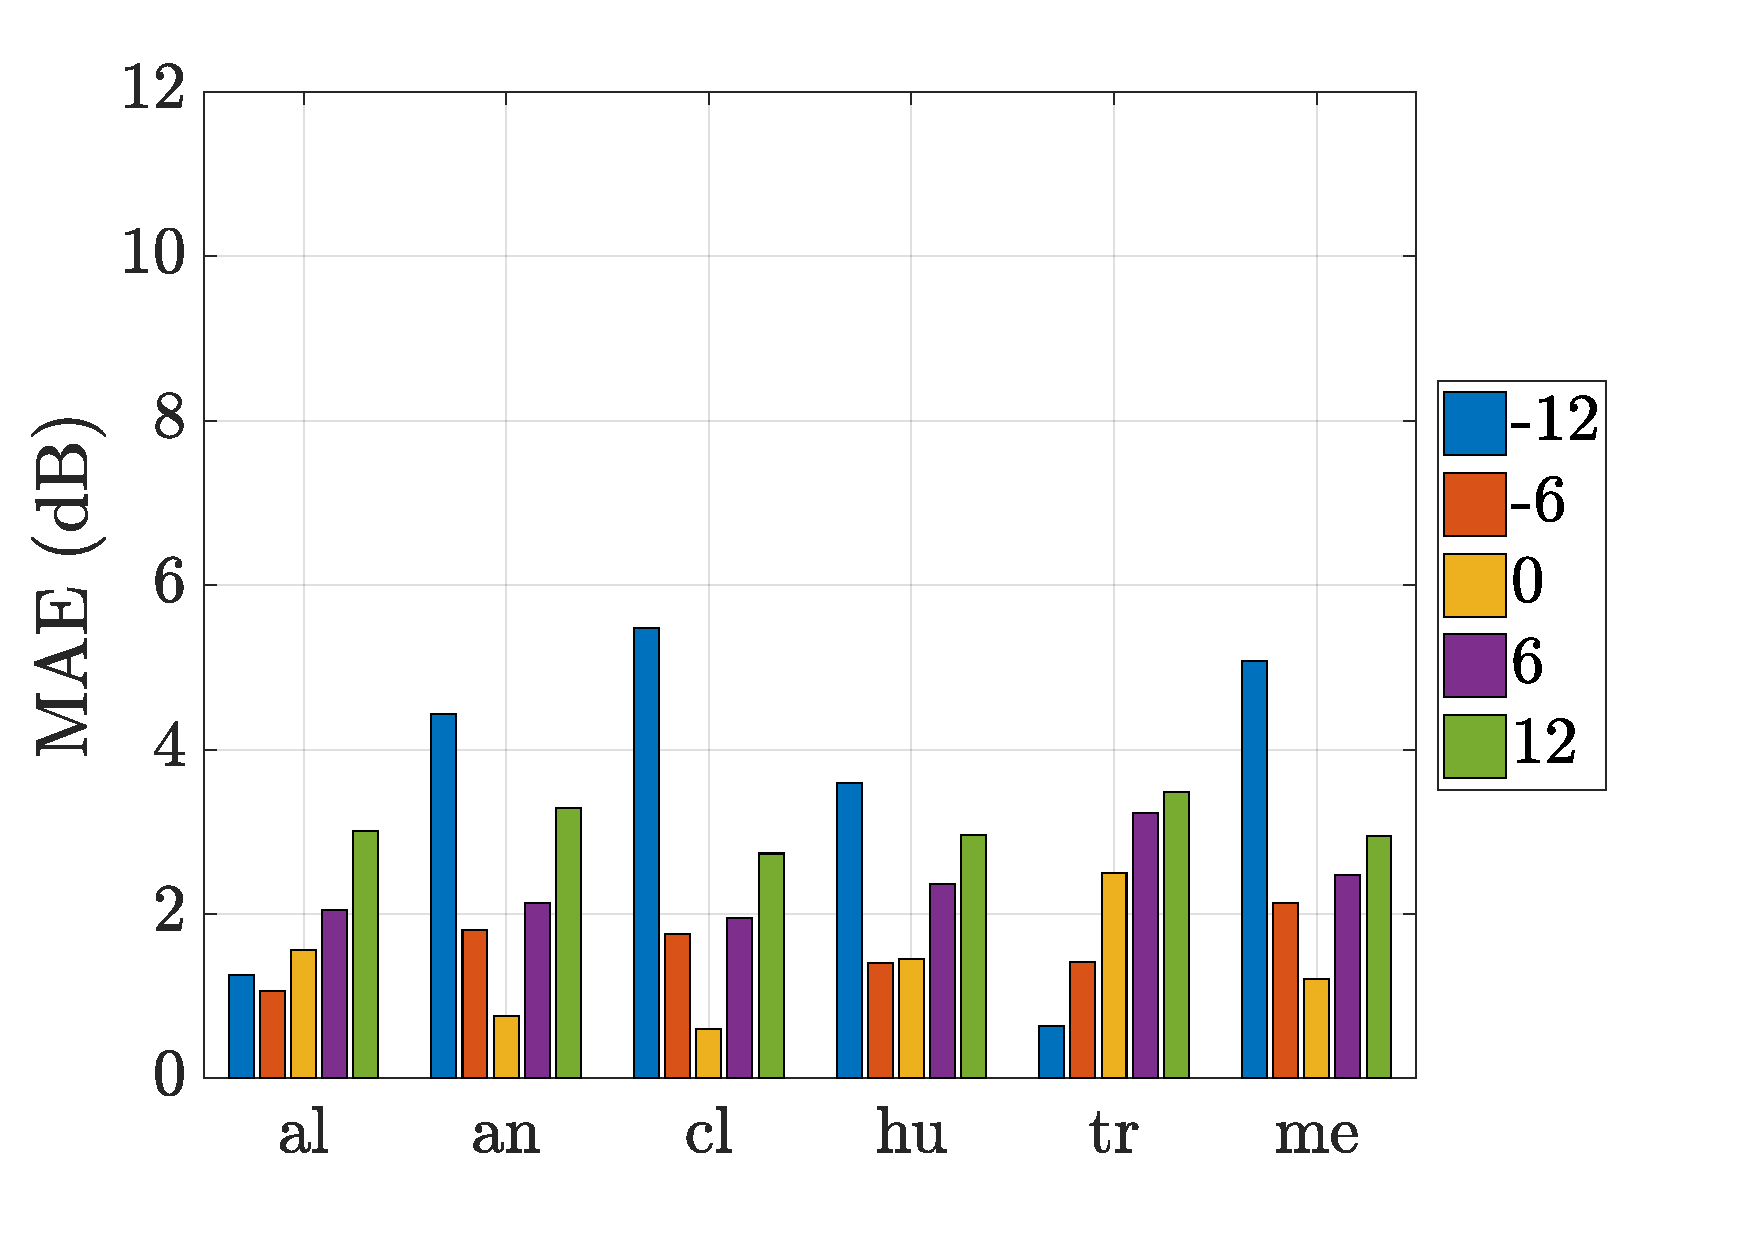
\includegraphics[width=\linewidth]{figures/semi-sup_bar.pdf}
        \caption{$MAE$ error for each $TIR$ and sub-class with Sem-NMF and $\beta$ = 2}
                \label{fig:TIR_class_semi}
    \end{subfigure}%
    \hfill
    \begin{subfigure}[t]{0.45\textwidth}
        \centering
        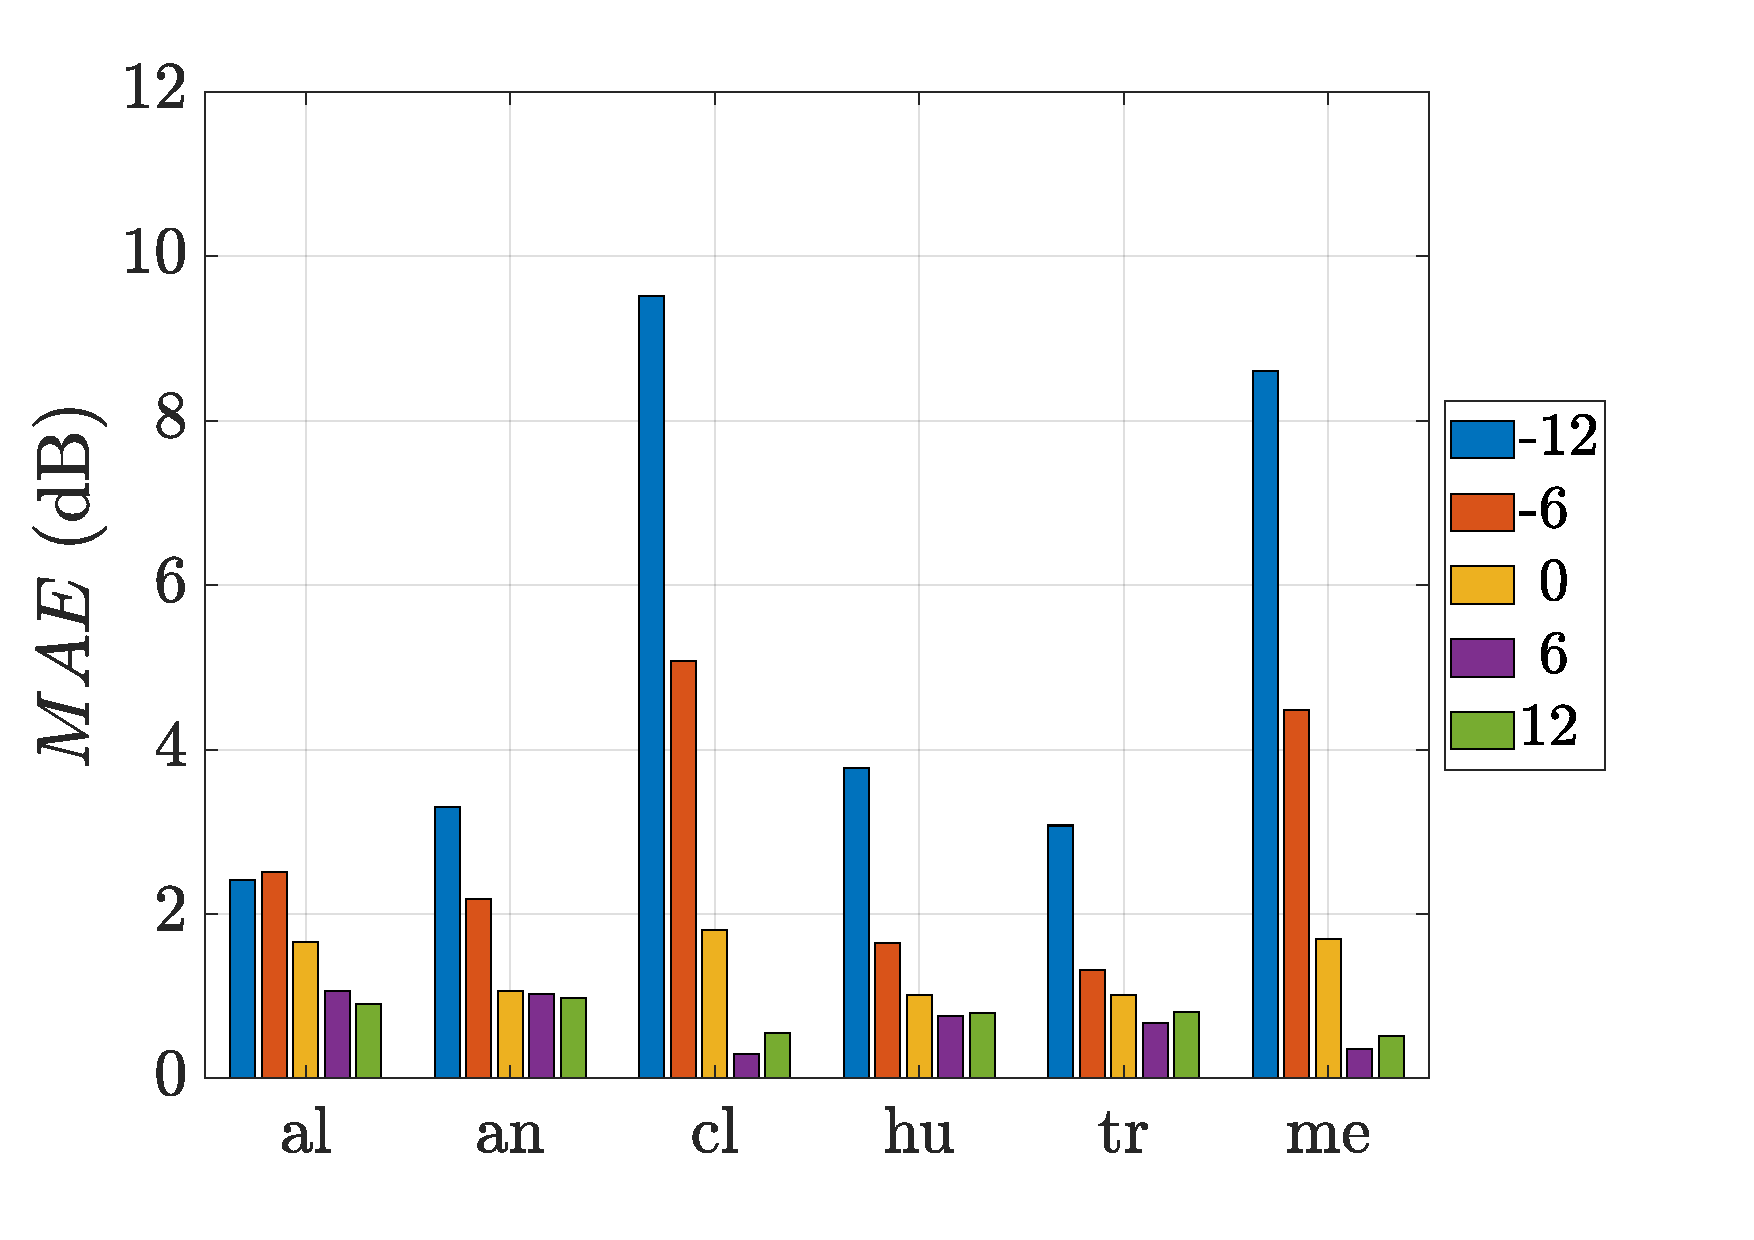
\includegraphics[width=\linewidth]{figures/TI_bar}
        \caption{$MAE$ error for each $TIR$ and sub-class with TI-NMF, $\beta$ = 1 and $t$ = 0.42}
        \label{fig:TIR_class_TI}
    \end{subfigure}
    \caption{$MAE$ error for each sub-class and each $TIR$ according to the the best results with the filter (\subref{fig:TIR_class_filter}) and each method (Sup-NMF (\subref{fig:TIR_class_sup}), Sem-NMF (\subref{fig:TIR_class_semi}) and TI-NMF (\subref{fig:TIR_class_TI}))}
    \label{fig:TIR_bar}
\end{figure*}

According to Table \ref{tab:results_TIR} and Figures \ref{fig:TIR_bar}, the behavior between the 3 versions of NMF differs. In the case of Sup-NMF, it fails to improve the filtering performances despite good results in high $TIR$. The errors are too important for low $TIR$ and this for all the sub-classes. This method reveals to be too rigid as $\mathbf{W}$ is composed of fixed traffic spectra. In the case of low $TIR$, in the aim to reduce the objective function, see eq. \ref{eq:min-D-WH}, traffic elements are used whatever the sound event in the  sound scene. In order to expose this issue, the case of a scene of the \textit{alert} sub-class is presented in Figure \ref{fig:lp_alert_-12}. Here when the \textit{alert} sub-class sounds, some traffic elements of $\mathbf{W}$ are activated. The \textit{alert} sub-class is then considered as traffic component generating a wrong estimation of the sound level, see Figure \ref{fig:lp_alert_-12}. This behavior disappears when the traffic component becomes predominant to the interfering class as in Figure \ref{fig:lp_alert_12}. Thus forcing the dictionary to be only traffic spectra is not a sufficient way to estimate correctly the traffic sound level, $\tilde{L}_{p,traffic}$.

Consequently, with the addition of a mobile part in the dictionary, $\mathbf{W_r}$, the semi-supervised approach  allows a better consideration of the interfering class in low $TIR$. It brings a significant decrease of the errors for low $TIR$ as it can be seen in Figure \ref{fig:TIR_class_semi}. The content of $\mathbf{W_r}$, in the case of an \textit{alert} sub-class is displayed in Figure \ref{fig:Y_alert-12}. The interfering class is easily integrated. The first element is mainly composed of high frequency bands which correspond to the car horns of the scene. This composition impacted directly the traffic sound level estimation as it can be seen in Figure \ref{fig:lp_alert_-12} where the elements of the dictionary dedicated to the traffic are no longer activated when the car horn is active.

\begin{figure*}[t]
    \centering
    \begin{subfigure}[t]{0.45\textwidth}
        \centering
        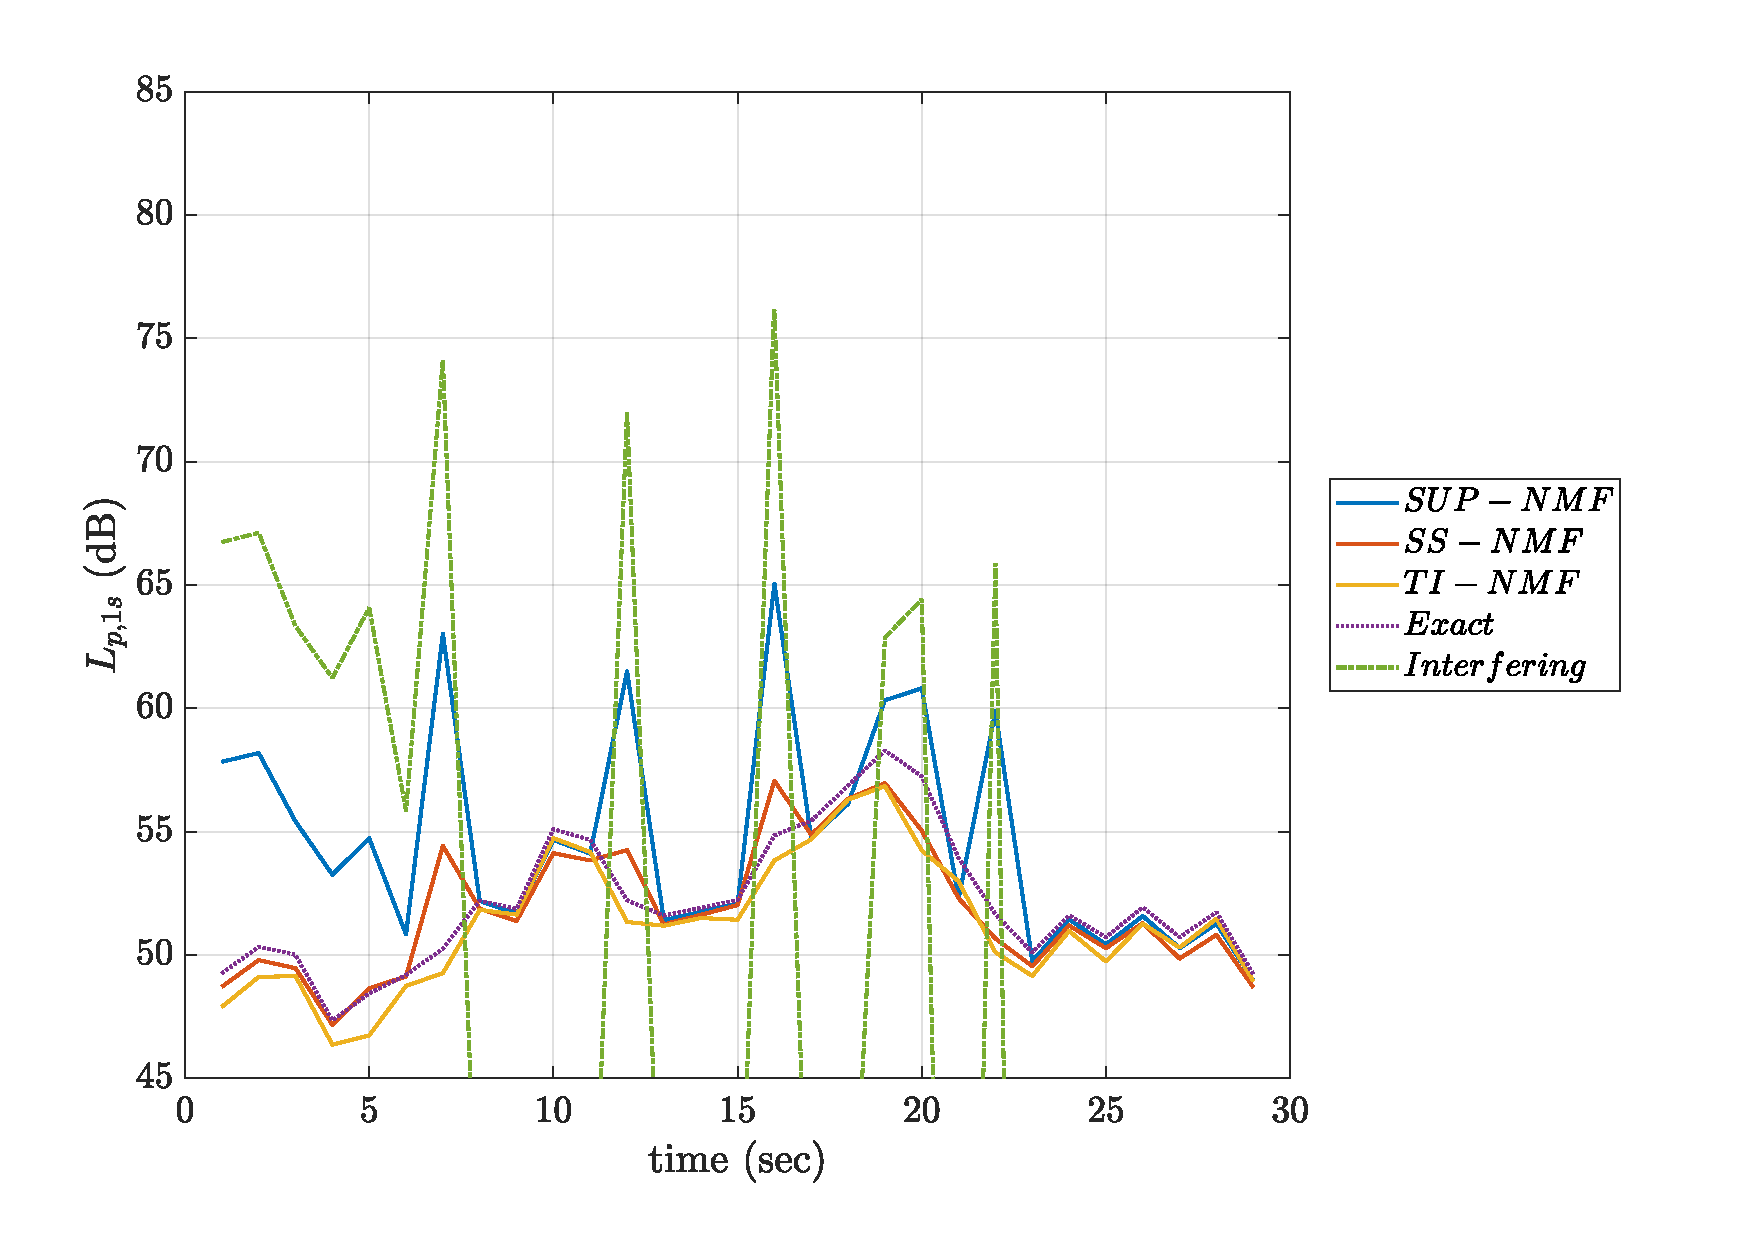
\includegraphics[width=\linewidth]{figures/NMF_Lp_alert-12.pdf}
        \caption{}
        \label{fig:lp_alert_-12}
    \end{subfigure}%
    \hfill
    \begin{subfigure}[t]{0.45\textwidth}
        \centering
        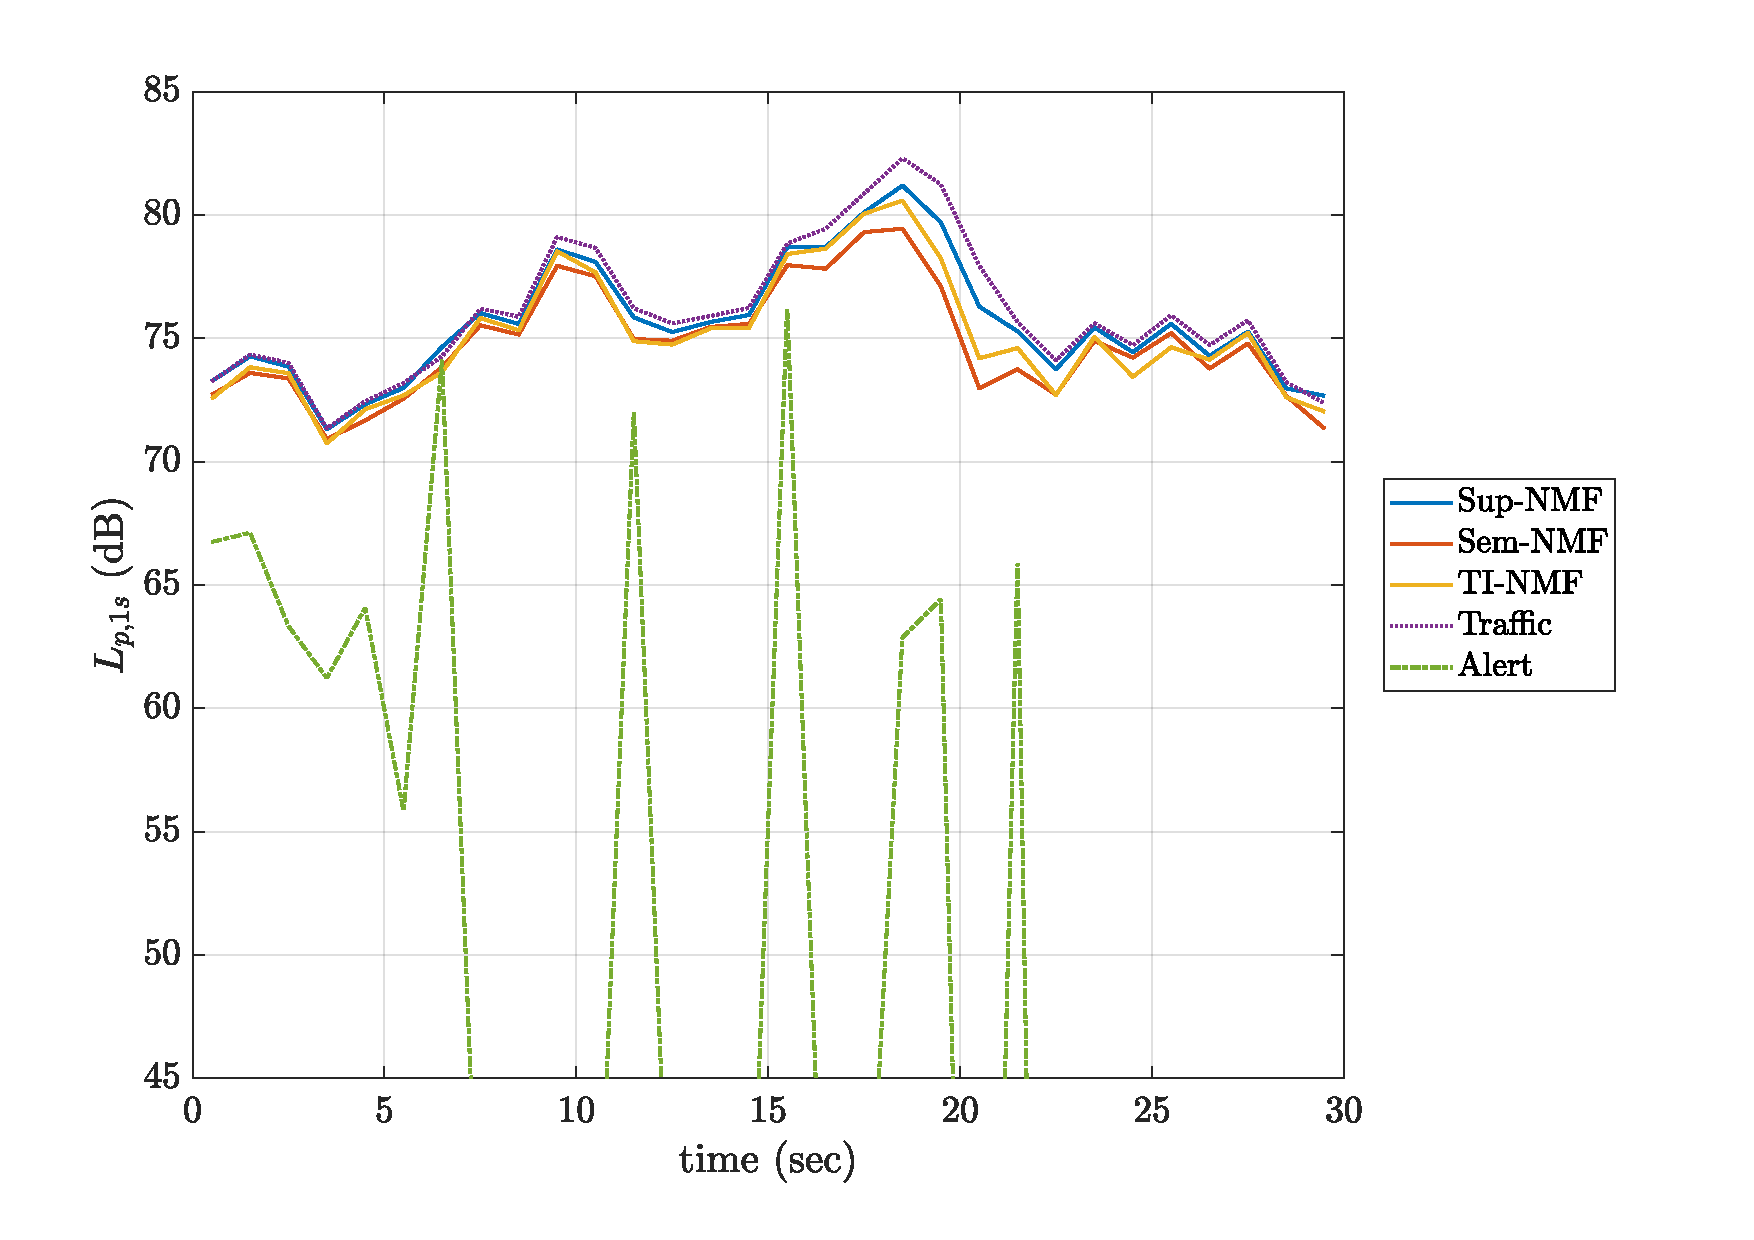
\includegraphics[width=\linewidth]{figures/NMF_Lp_alert12.pdf}
        \caption{}
        \label{fig:lp_alert_12}
    \end{subfigure}

    \caption{1 second equivalent sound pressure level of an \textit{alert} sub-class scene for supervised NMF ($\beta$ = 2, $K$ = 50, $w_t$ = 0.5 s), semi-supervised ($\beta$ = 2, $K$ = 100, $w_t$ = 0.5 s) and thresholded initialized ($\beta$ = 1, $K$ = 200, $w_t$ = 0.5 s, $t$ = 0.42) at $TIR = -12$ dB(\subref{fig:lp_alert_-12}) and $TIR$ = 12 dB (\subref{fig:lp_alert_12})}
    \label{fig:lp_alert}
\end{figure*}

However, the relatively high degree of freedom of Sem-NMF are restrictive for high $TIR$ as the errors exceed 2 dB for all sub-classes and increase with $TIR$ = 6 dB and 12 dB. In order to reduce $D(\mathbf{V} \vert \vert \mathbf{WH}$), without constraint, Sem-NMF is free to include traffic components in $\mathbf{W_r}$. Consequently, this behavior decreases the quality of the reconstruction of the traffic component. In Figure \ref{fig:Y_alert_12} for $TIR=12$ dB, the high frequency components of car horns have disappeared for the benefit of low frequency content. Consequently, the traffic sound level estimation is then underestimated as in Figure \ref{fig:lp_alert_12}. \\

\begin{figure}
    \centering
    \begin{subfigure}[t]{0.45\textwidth}
        \centering
        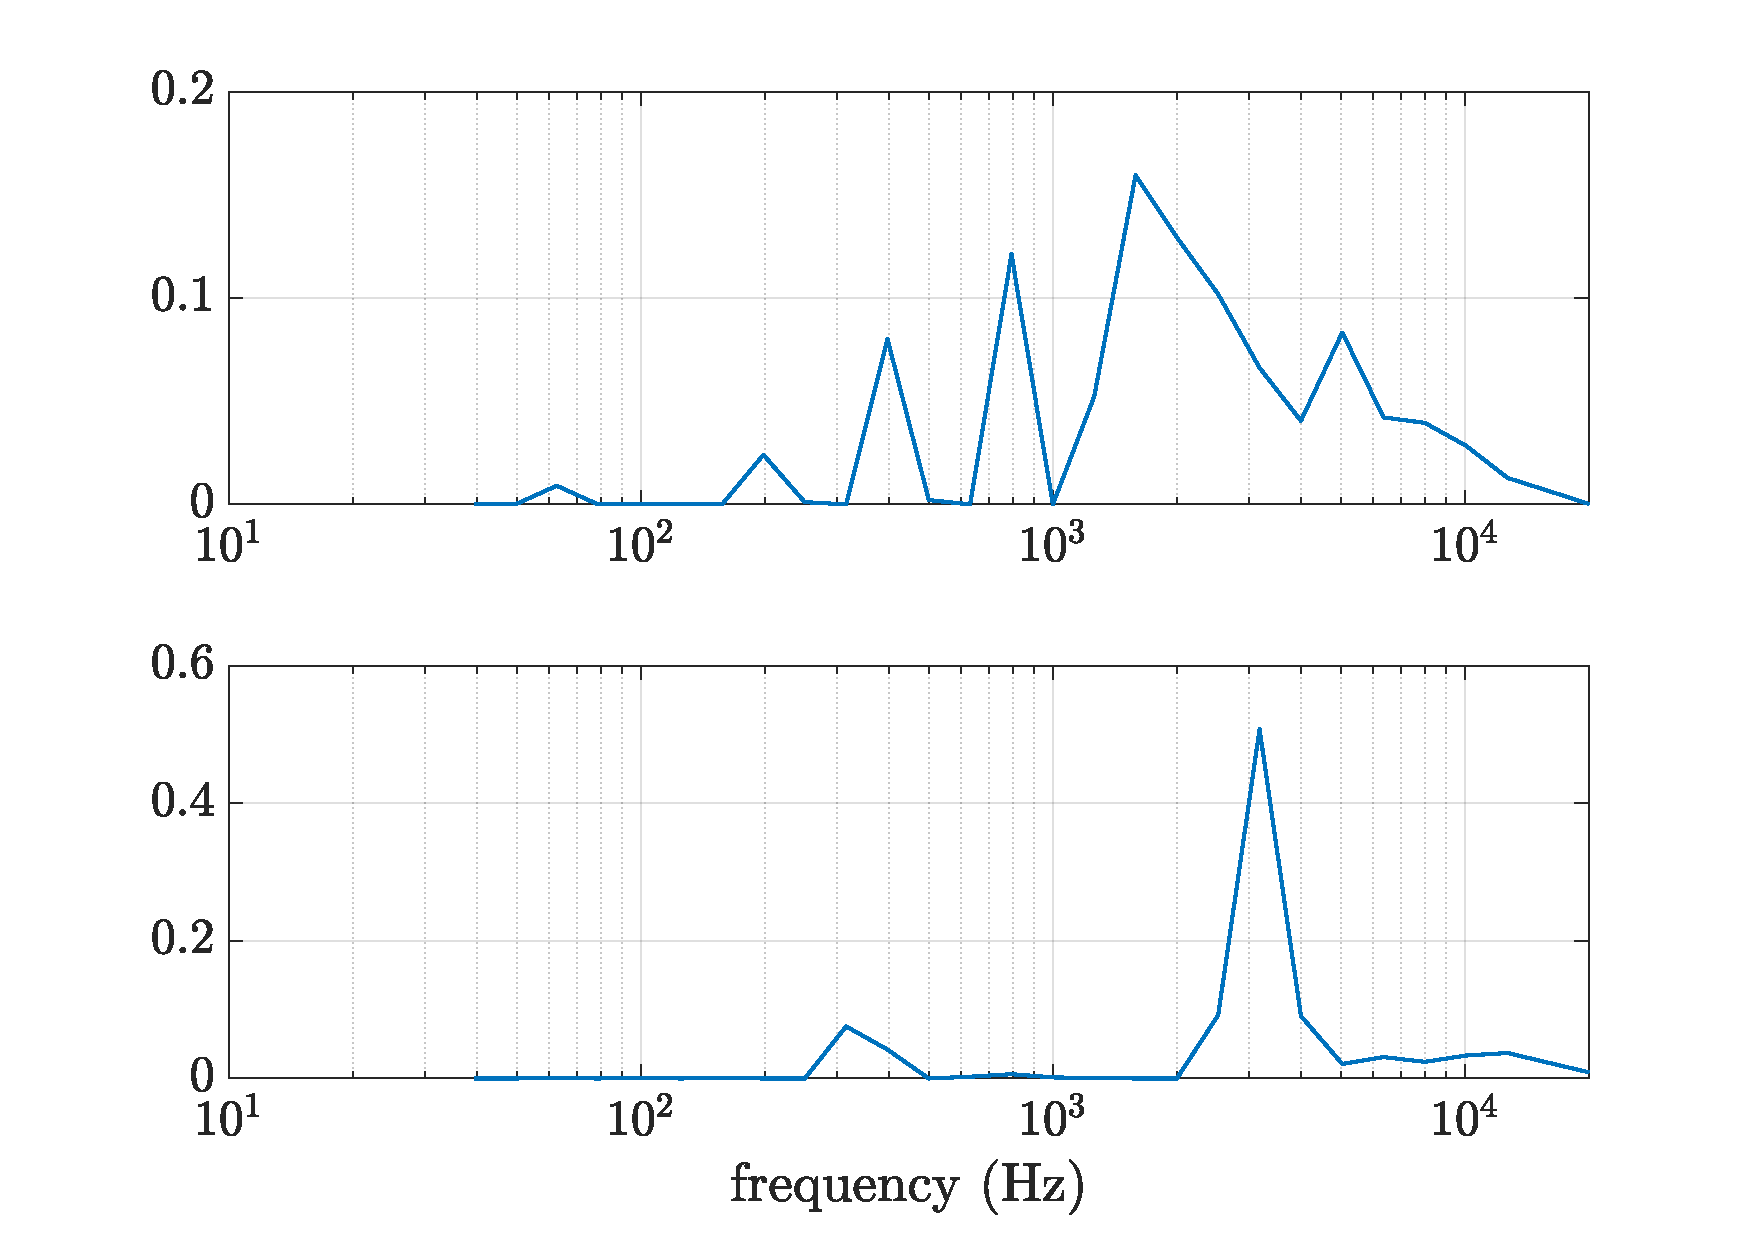
\includegraphics[width=\linewidth]{figures/Y_alert_-12.pdf}
        \caption{}
        \label{fig:Y_alert-12}
    \end{subfigure}
    \vfill
    \begin{subfigure}[t]{0.45\textwidth}
        \centering
        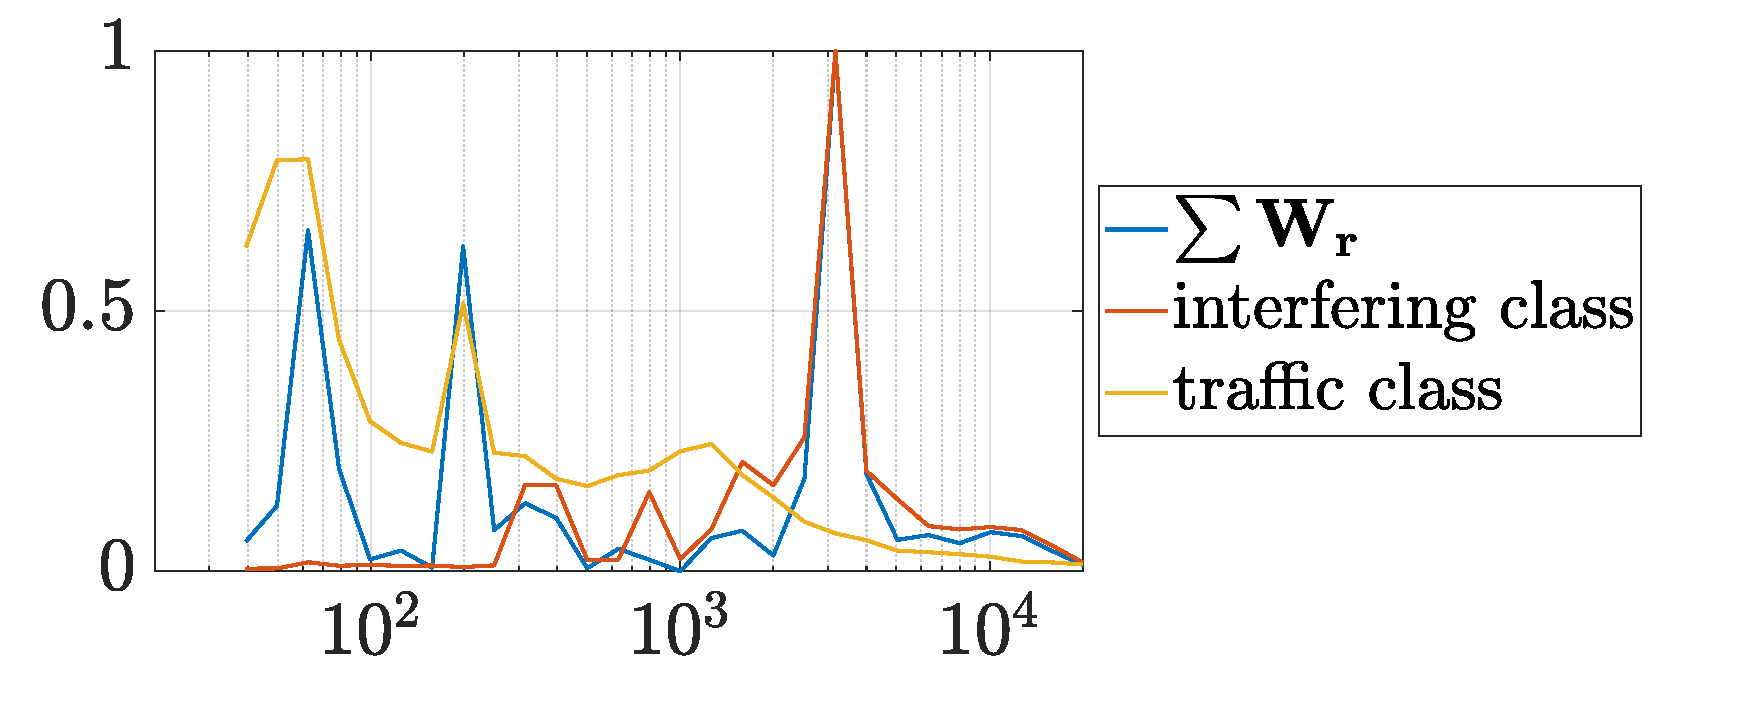
\includegraphics[width=\linewidth]{figures/Y_alert_12.pdf}
        \caption{}
		\label{fig:Y_alert_12}
    \end{subfigure}
    \caption{Comparison between the sum of the 2 elements of $\mathbf{W_r}$ with the spectra of the interfering and traffic classes for an \textit{alert} scene for $TIR$ = -12 dB (\subref{fig:Y_alert-12}) and $TIR$ = 12 dB (\subref{fig:Y_alert_12}) with $\beta = 2$, $K = 100$ and $w_t$ = 0.5 s (normalized amplitudes)}
\end{figure}


Finally, TI-NMF with a threshold $t = 0.42$ and $\beta$ = 1, offers the lowest average error (Table \ref{tab:results}). Unlike Sup-NMF, where $\mathbf{W}$ is fixed, and Sem-NMF, where only $\mathbf{W_r}$ is updated, TI-NMF updates $\mathbf{W}$ entirely to adjust prior knowledge to the scene under evaluation so as to adapt to the different sound environments. The closest elements of the traffic component defined in $\mathbf{W_0}$ are then extracted to deduce the traffic signal. In Figure \ref{fig:dist_-12_12}, the similarity $D_{\theta}(\mathbf{W_0}||\mathbf{W})$ is displayed for 3 sub-classes and $TIR$ = [-12, 12] dB.

\begin{figure}[t]
    \centering
    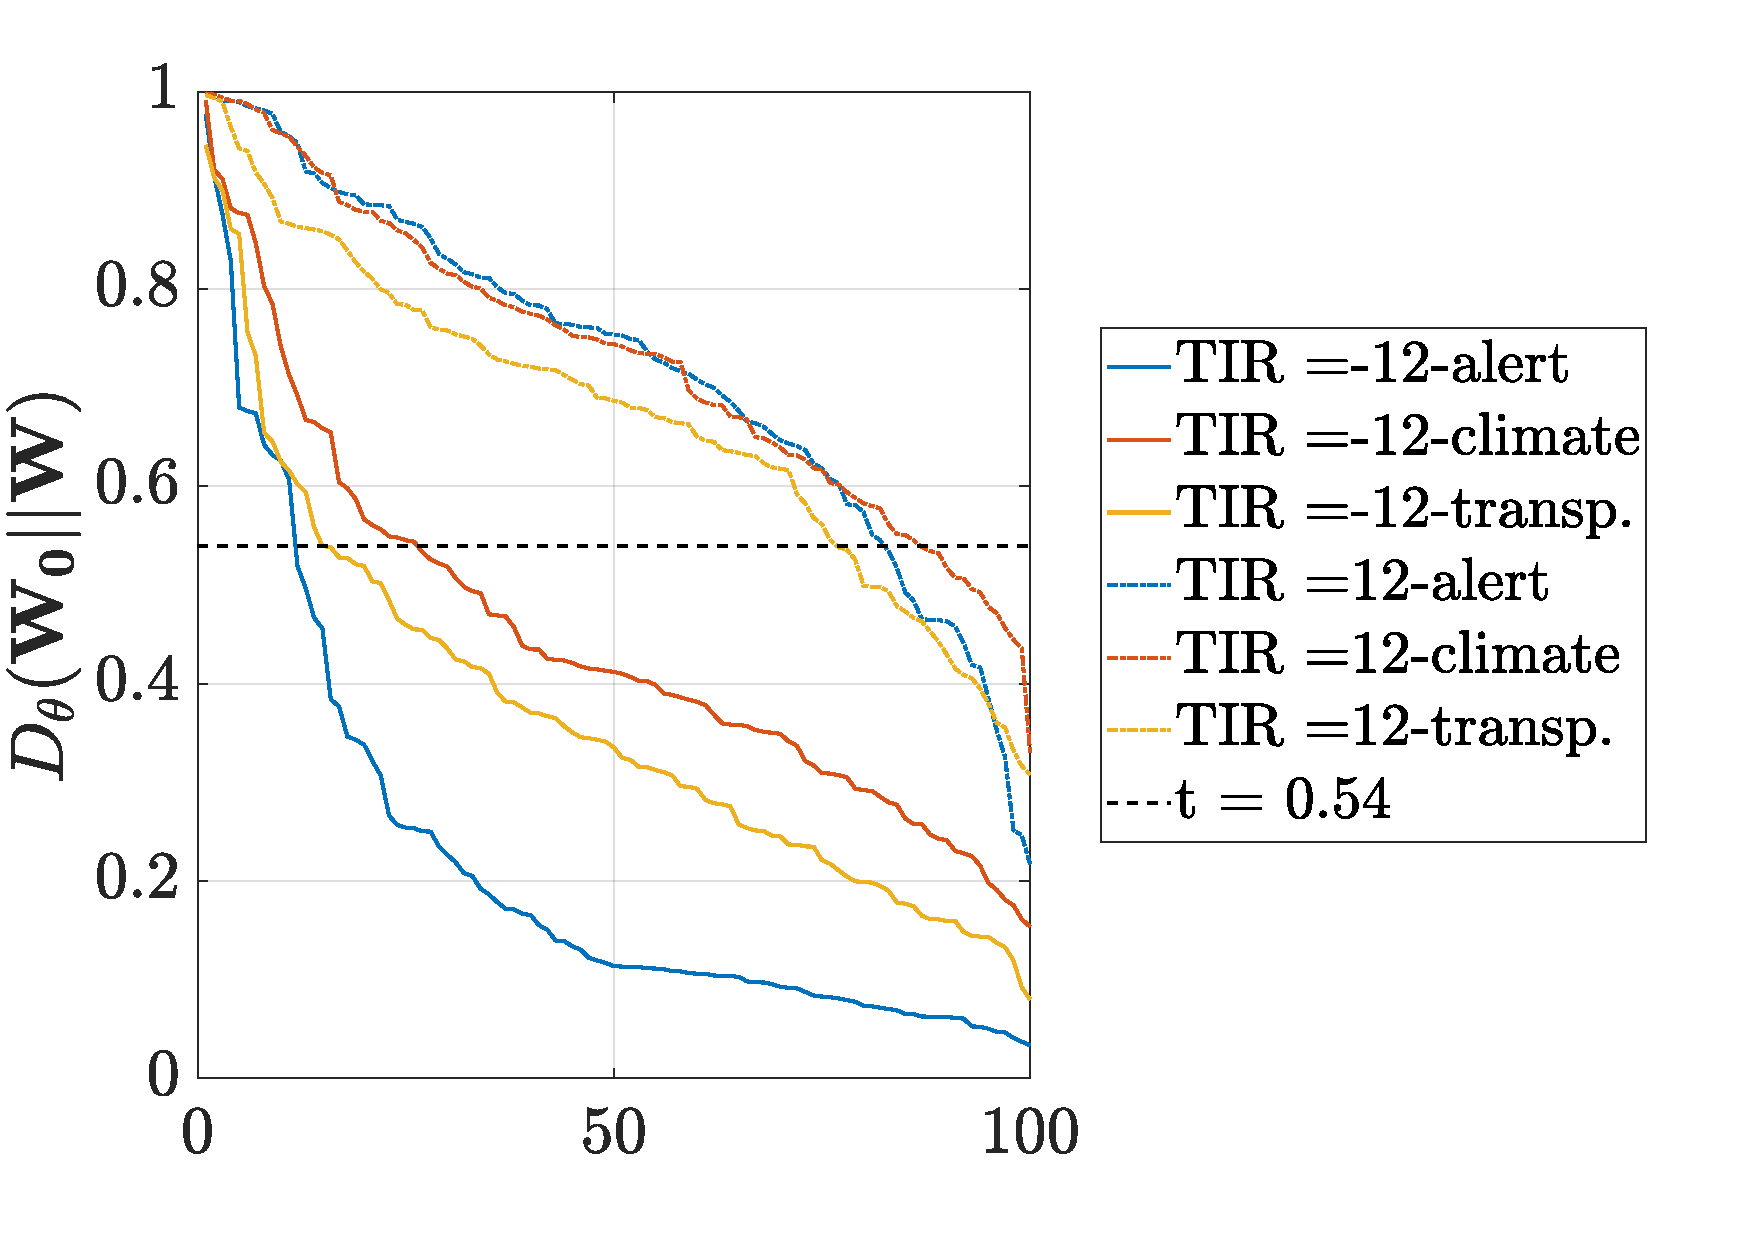
\includegraphics[width=.8\linewidth]{figures/dist_-12_12.pdf}
    \caption{Example of the similarity $D_{\theta}\left( \mathbf{W_0} \vert \vert \mathbf{W}\right)$ for different sub-classes and for two $TIR$ (-12 dB and 12 dB) and with the threshold $t$ = 0.42 ($\beta$ = 1, $K$ = 200 and $w_t$ = 0.5 s)}
    \label{fig:dist_-12_12}
\end{figure}

For low $TIR$, as the traffic sound class is not predominant, the final dictionary strongly differs from the $\mathbf{W_0}$. With the thresholding, only a reduced number of basis vectors are considered as traffic components. In comparison to supervised results, this approach reduces significantly the error for the \textit{human} and \textit{transport} sub-classes.  However, for \textit{climate} and \textit{mechanics}, the errors remain important as these interfering classes have similar spectral profiles when compared to traffic ones.

For high $TIR$, as the traffic is the main sound source, the similarity of the initial dictionary and $\mathbf{W}$ is higher what allows retaining more elements as traffic components and then decreases the error (< 1 dB). The kept elements are then more suited to the scenes than a fixed dictionary. The error for these $TIR$ is then due to the thresholding which put aside some elements that are nevertheless related to the traffic component. With a low threshold, it is possible to decrease the error. For $TIR$ = 12 dB, the average error on all the sub-classes is 0.22 ($\pm$ 0.08) dB with $t$ = 0.30. In opposite for $TIR$ = -12 dB, it is better to choose a high threshold $t$ = 0.55, the error decrease to 4.46 $\pm$ 1.66. In order to generalize this method and having no prior knowledge on the urban environment, the chosen threshold $t$ is then fixed to $t$ = 0.42 and is the one that best balanced these opposite cases.

\section{Conclusion}

In this work the non negative metric factorization framework  was used to estimate the road traffic sound level in urban sound mixtures. It is a well suited approach to these sound environments because it easily takes into account the overlap between the multiple sound sources present in the cities and it is adapted to monophonic sensor networks. Different versions of NMF have been studied as a supervised and semi-supervised approach. On a large corpus of sounds, the supervised approach proves to be too restrictive to be adapted to different sound environments whereas the semi-supervised approach has, on the contrary, too many degrees of freedom on the mobile dictionary $\mathbf{W_r}$, decreasing its performance especially when the traffic is predominant. The proposed approach, named threshold initialized NMF achieves the lowest average error. With this method, the $\mathbf{W}$ is initialized with road traffic spectra, updated and the dictionary elements that are similar to the road traffic spectra are then extracted by hard thresholding. 
A major advantage of the proposed approach is that it is not designed for a specific source. Even though the experiments described in this paper focused on traffic sounds, changing the dictionary to contain bird sounds would lead to an estimator of the presence of birds. Extending the apporach to other sources is thus of intetrest for future research. Also, performance improvement could be achieved by the addition of constraints such as sparsness \cite{hoyer2004non} and smoothness \cite{virtanen_monaural_2007} of the low rank matrices.

The experimental protocol and the evaluated estimators have been implemented with the Matlab software. For reproducible purposes, the code is available online\footnote{\url{https://github.com/jean-remyGloaguen/article2017EstimationAmbiance}}. The evaluation database composed of multiple samples of urban sounds is also made available for the research community with interest in detection, separation and recognition tasks of urban sound sources.


\footnotesize
\bibliographystyle{unsrt}
\bibliography{bibliographie_sensors}

\end{document}
